\documentclass[acmtog]{acmart}

\AtBeginDocument{%
  \providecommand\BibTeX{{%
    Bib\TeX}}}

\setcopyright{licensedothergov}

\usepackage[T1]{fontenc} % Поддержка кодировки шрифтов
\usepackage[utf8]{inputenc} % Поддержка UTF-8 для ввода символов
\usepackage[english,russian]{babel} % Поддержка русского и английского языков

\acmJournal{TOG}

\acmSubmissionID{685}



\citestyle{acmauthoryear}

\usepackage{subcaption}
\usepackage{multirow}
\usepackage{xcolor,colortbl}
\usepackage{algorithm}
\usepackage{algpseudocode}
\usepackage{tikz}
\usepackage{graphicx}
\usetikzlibrary{spy,backgrounds}
\usepackage{soul}

\usepackage[percent]{overpic}

\DeclareGraphicsRule{.ai}{pdf}{.ai}{}

\newcommand{\GD}[1]{\textcolor{red}{#1}}
\newcommand{\TODO}[1]{}
\newcommand{\GK}[1]{\textcolor{blue}{GK: #1}}
\newcommand{\BK}[1]{\textcolor{cyan}{BK: #1}}
\newcommand{\TL}[1]{\textcolor{purple}{TL: #1}}

\setcopyright{licensedothergov}
\acmYear{2023} \acmVolume{42} \acmNumber{4} \acmArticle{1} \acmMonth{8} \acmPrice{15.00} \acmDOI{10.1145/3592433}

\begin{document}

\title{3D Gaussian Splatting для рендеринга радиусных полей в реальном времени}


\author{Бернхард Кербл}
\orcid{0000-0002-5168-8648}
\authornote{Оба автора внесли равный вклад в статью.}
\email{bernhard.kerbl@inria.fr}
\affiliation{%
    \institution{Inria, Universit\'e C\^ote d'Azur}
    \country{Франция}
}
\author{Георгиос Копанас}
\orcid{0009-0002-5829-2192}
\authornotemark[1]
\email{georgios.kopanas@inria.fr}
\affiliation{%
    \institution{Inria, Universit\'e C\^ote d'Azur}
    \country{Франция}
}
\author{Томас Леймкюлер}
\orcid{0009-0006-7784-7957}
\email{thomas.leimkuehler@mpi-inf.mpg.de}
\affiliation{%
    \institution{Max-Planck-Institut f\"{u}r Informatik}
    \country{Германия}
}
\author{Джордж Дреттакис}
\orcid{0000-0002-9254-4819}
\email{george.drettakis@inria.fr}
\affiliation{%
    \institution{Inria, Universit\'e C\^ote d'Azur}
    \country{Франция}
}

\def\Dg{DG}



\newcommand{\ADDITION}[1]{#1}
\newcommand{\REMOVAL}[1]{}
\newcommand{\CORRECTION}[2]{#2}


\begin{abstract}
Методы радиусных полей недавно произвели революцию в синтезе новых видов сцен, захваченных с помощью множества фотографий или видео. Однако достижение высокого визуального качества по-прежнему требует нейронных сетей, которые дороги в обучении и рендеринге, а недавние более быстрые методы неизбежно жертвуют скоростью ради качества. Для неограниченных и полных сцен (в отличие от изолированных объектов) и рендеринга с разрешением 1080p ни один из текущих методов не может достичь частоты вывода изображений в реальном времени. Мы представляем три ключевых элемента, которые позволяют нам достичь передового визуального качества, сохраняя при этом конкурентные времена обучения и, что важно, обеспечивают высококачественный синтез новых видов в реальном времени ($\geq30$~fps) с разрешением 1080p. Во-первых, начиная со скудных точек, созданных во время калибровки камеры, мы представляем сцену с помощью 3D Гауссиан, сохраняя желаемые свойства непрерывных объемных радиусных полей для оптимизации сцены, избегая при этом ненужных вычислений в пустом пространстве; Во-вторых, мы выполняем чередующуюся оптимизацию/контроль плотности 3D Гауссиан, особенно оптимизируя анизотропную ковариацию для достижения точного представления сцены; В-третьих, мы разрабатываем быстрый алгоритм рендеринга с учетом видимости, который поддерживает анизотропное сплаттинг и ускоряет как обучение, так и позволяет рендеринг в реальном времени. Мы демонстрируем передовое визуальное качество и рендеринг в реальном времени на нескольких установленных наборах данных.
\end{abstract}

\begin{CCSXML}
    <ccs2012>
    <concept>
    <concept_id>10010147.10010371.10010372.10010373</concept_id>
    <concept_desc>Вычислительные методологии~Растеризация</concept_desc>
    <concept_significance>500</concept_significance>
    </concept>
    <concept>
    <concept_id>10010147.10010257.10010293</concept_id>
    <concept_desc>Вычислительные методологии~Подходы машинного обучения</concept_desc>
    <concept_significance>300</concept_significance>
    </concept>
    <concept>
    <concept_id>10010147.10010371.10010396.10010400</concept_id>
    <concept_desc>Вычислительные методологии~Модели на основе точек</concept_desc>
    <concept_significance>500</concept_significance>
    </concept>
    <concept>
    <concept_id>10010147.10010371.10010372</concept_id>
    <concept_desc>Вычислительные методологии~Рендеринг</concept_desc>
    <concept_significance>500</concept_significance>
    </concept>
    </ccs2012>
\end{CCSXML}

\ccsdesc[500]{Вычислительные методологии~Рендеринг}
\ccsdesc[500]{Вычислительные методологии~Модели на основе точек}
\ccsdesc[500]{Вычислительные методологии~Растеризация}
\ccsdesc[500]{Вычислительные методологии~Подходы машинного обучения}

\keywords{синтез новых видов, радиусные поля, 3D гауссианы, рендеринг в реальном времени}

\begin{teaserfigure}
    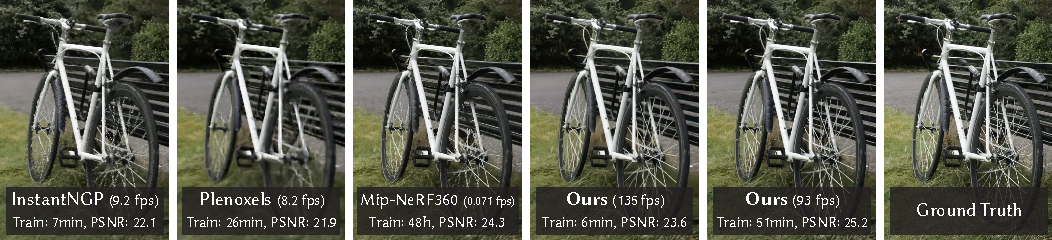
\includegraphics[width=\textwidth]{figures/teaser/teaser_02.pdf}
    \caption{
    \label{fig:teaser}
    Наш метод достигает рендеринга радиусных полей в реальном времени с качеством, равным предыдущему методу с наилучшим качеством ~\cite{barron2022mipnerf360}, требуя при этом времени оптимизации только конкурентного с самыми быстрыми предыдущими методами~\cite{plenoxels,mueller2022instant}.
    Ключом к этой производительности является новое представление сцены с помощью 3D Гауссиан в сочетании с дифференцируемым рендером в реальном времени, который обеспечивает значительное ускорение как оптимизации сцены, так и синтеза новых видов.
    Обратите внимание, что для сравнимого времени обучения с InstantNGP ~\cite{mueller2022instant} мы достигаем качество, аналогичное их; хотя это максимальное качество, которое они достигают, обучаясь 51 минуту, мы достигаем передового качества, даже немного лучше, чем Mip-NeRF360~\cite{barron2022mipnerf360}. %
    }
    \Description[TeaserFigure]{TeaserFigure}
\end{teaserfigure}
\maketitle


\section{Введение}

Сетки и точки являются наиболее распространенными представлениями 3D-сцен, поскольку они явные и хорошо подходят для быстрой растеризации на базе GPU/CUDA. 
В отличие от них, современные методы Нейронных Радиусных Полей (NeRF) основываются на непрерывных представлениях сцен, обычно оптимизируя многослойный перцептрон (MLP) с использованием объемного трассирования лучей для синтеза новых видов захваченных сцен. Аналогично, самые эффективные на данный момент решения радиусных полей строятся на непрерывных представлениях, интерполируя значения, хранящиеся, например, в воксельных~\cite{plenoxels} или хеш-сетках~\cite{mueller2022instant}, или точках~\cite{xu2022point}.
Хотя непрерывная природа этих методов способствует оптимизации, стохастическая выборка, необходимая для рендеринга, является дорогостоящей и может привести к шуму.
Мы представляем новый подход, который сочетает в себе лучшее из обоих миров: наши 3D Гауссианы позволяют проводить оптимизацию с качеством визуализации на уровне современного уровня (SOTA) и конкурентным временем обучения,
в то время как наше решение на основе тайлового сплаттинга обеспечивает рендеринг в реальном времени с SOTA качеством для разрешения 1080p на нескольких ранее опубликованных наборах данных~\cite{knapitsch2017tanks,hedman2018deep,barron2022mipnerf360} (см. Рис.~\ref{fig:teaser}).


Наша цель — позволить рендеринг в реальном времени для сцен, захваченных с помощью множества фотографий, и создать представления с временем оптимизации, таким же быстрым, как у самых эффективных предыдущих методов для типичных реальных сцен.
Недавние методы достигают быстрого обучения~\cite{plenoxels,mueller2022instant}, но испытывают трудности в достижении качества визуализации, получаемого текущими SOTA NeRF методами, т. е., Mip-NeRF360~\cite{barron2022mipnerf360}, который требует до 48 часов времени обучения. Быстрые, но менее качественные методы радиусных полей могут достигать интерактивного времени рендеринга в зависимости от сцены (10–15 кадров в секунду), но не достигают рендеринга в реальном времени \CORRECTION{($\geq$ 30~fps)}{} при высоком разрешении.

Наше решение строится на трех основных компонентах. Мы сначала вводим \emph{3D Гауссианы} как гибкое и выразительное представление сцены.
Мы начинаем с того же входного сигнала, что и предыдущие методы, похожие на NeRF, т.е., камеры, откалиброванные с помощью Structure-from-Motion (SfM) \cite{snavely2006photo}, и инициализируем набор 3D Гауссиан с использованием разреженного облака точек, которое создается бесплатно как часть процесса SfM. В отличие от большинства решений на основе точек, которые требуют данных Многовидового Стерео (MVS)~\cite{aliev20,kopanas21,ruckert22}, мы достигаем высококачественных результатов только с использованием точек SfM на входе. Отметим, что для NeRF-синтетического набора данных наш метод достигает высокого качества даже при случайной инициализации.
Мы показываем, что 3D Гауссианы являются отличным выбором, поскольку это дифференцируемое объемное представление, но их также можно очень эффективно растеризовать, проецируя их в 2D и применяя стандартное $\alpha$-смешивание, используя ту же модель формирования изображения, что и NeRF.
Второй компонент нашего метода заключается в оптимизации свойств 3D Гауссиан — 3D позиции, непрозрачности $\alpha$, анизотропной ковариации и коэффициентов сферических гармоник (SH) — чередующихся с шагами адаптивного контроля плотности, где мы добавляем и иногда удаляем 3D Гауссианы во время оптимизации. Процедура оптимизации создает достаточно компактное, неструктурированное и точное представление сцены (1–5 миллионов Гауссиан для всех протестированных сцен).
Третий и последний элемент нашего метода — это наше решение для рендеринга в реальном времени, которое использует быстрые алгоритмы сортировки GPU и вдохновлено тайловой растеризацией, следуя недавним работам~\cite{Lassner_2021_CVPR}. Однако благодаря нашему представлению 3D Гауссиан мы можем выполнять анизотропное сплатирование, учитывая порядок видимости — благодаря сортировке и $\alpha$-смешиванию — и обеспечивать быстрый и точный обратный проход, отслеживая прохождение стольких отсортированных сплатов, сколько необходимо.



\noindent
Подводя итог, мы предоставляем следующие вклады:

    
- Введение анизотропных 3D Гауссиан как высококачественного, неструктурированного представления радиусных полей.
    
- Метод оптимизации свойств 3D Гауссиан, чередующийся с адаптивным контролем плотности, создающий высококачественные представления для захваченных сцен.
    
- Быстрый, дифференцируемый подход к рендерингу для GPU, учитывающий видимость, позволяющий анизотропное сплатирование и быстрое обратное распространение для достижения высококачественного синтеза новых видов.


\noindent
Наши результаты на ранее опубликованных наборах данных показывают, что мы можем оптимизировать наши 3D Гауссианы из многовидовых захватов и достичь качества, равного или лучшего, чем у лучших предыдущих неявных методов радиусных полей. Мы также можем достичь скоростей обучения и качества, аналогичных самым быстрым методам, и, что важно, предоставить первый \emph{рендеринг в реальном времени} с высоким качеством для синтеза новых видов.
\section{Связанные работы}
Мы сначала кратко обозреваем традиционную реконструкцию, затем обсуждаем методы рендеринга на основе точек и радиусных полей, рассматривая их сходство; радиусные поля — это обширная область, поэтому мы фокусируемся только на непосредственно связанных работах. 
Для полного охвата области, пожалуйста, см. отличные недавние обзоры~\cite{tewari2022advances,xie2022neural}.
\subsection{Традиционная реконструкция сцен и рендеринг}
Первые подходы к синтезу новых видов были основаны на световых полях, сначала плотно семплированных~\cite{gortler1996lumigraph,levoy1996light}, а затем позволяющих неструктурированный захват~\cite{buehler2001unstructured}. Появление метода Structure-from-Motion (SfM)~\cite{snavely2006photo} открыло новую область, где коллекция фотографий могла использоваться для синтеза новых видов. SfM оценивает разреженное облако точек во время калибровки камеры, которое изначально использовалось для простой визуализации 3D пространства. Последующие многовидовые стерео методы (MVS) привели к появлению впечатляющих алгоритмов полной 3D реконструкции за прошедшие годы~\cite{goesele2007multi}, что позволило разработать несколько алгоритмов синтеза видов \cite{eisemann2008floating, chaurasia2013depth, hedman2018deep,kopanas21}.
Все эти методы \emph{репроектируют} и \emph{смешивают} входные изображения в камеру нового ракурса, используя геометрию для управления этой репроекцией. Эти методы давали отличные результаты во многих случаях, но обычно не могут полностью восстановиться после нереконструированных областей или из-за «чрезмерной реконструкции», когда MVS создает несуществующую геометрию.
Недавние алгоритмы нейронного рендеринга ~\cite{tewari2022advances} значительно уменьшают такие артефакты и избегают огромной стоимости хранения всех входных изображений на GPU, превосходя эти методы по большинству параметров.
\subsection{Нейронный рендеринг и радиусные поля}
Глубокие методы обучения были внедрены на ранних этапах для синтеза новых видов ~\cite{zhou2016view, flynn2016deepstereo}; сверточные нейронные сети (CNN) использовались для оценки весов смешивания~\cite{hedman2018deep}, или для решений в текстурном пространстве \cite{thies2019deferred,riegler2020free}. Использование геометрии, основанной на MVS, является основным недостатком большинства этих методов; кроме того, использование CNN для окончательного рендеринга \ADDITION{часто} приводит \REMOVAL{к частому} временному мерцанию.
Объемные представления для синтеза новых видов были инициированы Soft3D~\cite{penner2017soft}; глубокие методы обучения, связанные с объемным трассированием лучей, были предложены позднее~\cite{sitzmann2019deepvoxels,henzler2019escaping}, основываясь на непрерывном дифференцируемом поле плотности для представления геометрии. Рендеринг с использованием объемного трассирования лучей имеет значительную стоимость из-за большого количества выборок, необходимых для запроса объема. Нейронные радиусные поля (NeRFs)~\cite{mildenhall2020nerf} ввели важную выборку и позиционное кодирование для повышения качества, но использовали большой многослойный перцептрон, что негативно влияло на скорость.
Успех NeRF привел к взрыву последующих методов, которые решают проблемы качества и скорости, часто вводя стратегии регуляризации; текущее состояние техники в качестве изображения для синтеза новых видов — это Mip-NeRF360~\cite{barron2022mipnerf360}. Хотя качество рендеринга выдающееся, время обучения и рендеринга остается чрезвычайно высоким; мы можем соответствовать или в некоторых случаях превзойти это качество, обеспечивая быстрое обучение и рендеринг в реальном времени.
Наиболее современные методы сосредоточились на более быстром обучении и/или рендеринге, главным образом за счет трех проектных решений: использования пространственных структур данных для хранения (нейронных) признаков, которые затем интерполируются во время объемного трассирования лучей, различных кодировок и емкости MLP. Такие методы включают
различные варианты дискретизации пространства~\cite{nglod-cvpr2021,plenoxels,yu2021plenoctrees,hedman2021snerg,chen2022mobilenerf,garbin2021fastnerf,Reiser2021ICCV,tensorf-eccv2022,wu2022snisr},
кодовые книги~\cite{takikawa2022variable},
и кодировки, такие как хеш-таблицы~\cite{mueller2022instant}, что позволяет использовать меньший MLP или полностью отказаться от нейронных сетей \cite{plenoxels,dvgo-cvpr2022}. %
Наиболее примечательными из этих методов являются InstantNGP~\cite{mueller2022instant}, который использует хеш-сетку и сетку занятости для ускорения вычислений и меньший MLP для представления плотности и внешнего вида;
и Plenoxels~\cite{plenoxels}, которые используют разреженную воксельную сетку для интерполяции непрерывного поля плотности и могут полностью обойтись без нейронных сетей. \CORRECTION{Они оба заменяют MLP, используемый для представления направленных эффектов, гораздо более быстрыми сферическими гармониками.}
{Оба они полагаются на сферические гармоники: первый для прямого представления направленных эффектов, второй для кодирования своих входных данных в цветовую сеть.}
Хотя оба предоставляют выдающиеся результаты, эти методы все еще могут испытывать трудности с эффективным представлением пустого пространства, отчасти зависящие от типа сцены/захвата. Кроме того, качество изображения в значительной степени ограничено выбором структурированных сеток, используемых для ускорения, а скорость рендеринга ограничивается необходимостью запрашивать множество выборок для данного шага трассировки лучей. Неупорядоченные, явные, дружественные к GPU 3D Гауссианы, которые мы используем, обеспечивают более быструю скорость рендеринга и лучшее качество \emph{без} нейронных компонентов.
\subsection{Рендеринг на основе точек и радиусные поля}
Методы на основе точек эффективно рендерят отсоединенные и неструктурированные геометрические образцы (например, облака точек)~\cite{gross2011point}. 
В самой простой форме рендеринг точек выборки \cite{Grossman1998PointSR} растеризует неструктурированный набор точек с фиксированным размером, для которого может быть использована нативная поддержка типов точек графических API \cite{SAINZ2004869} или параллельная программная растеризация на GPU \cite{10.1145/3543863, laine2011high}. Будучи верным исходным данным, рендеринг точек выборки страдает от дыр, вызывает алиасинг и является строго разрывным. Семинальная работа по качественному рендерингу на основе точек решает эти проблемы путем "сплаттинга" точечных примитивов с протяженностью больше пикселя, например, круглых или эллиптических дисков, эллипсоидов или сурфелей \cite{10.1145/383259.383300, 10.5555/2386366.2386369, Ren2002ObjectSE, 10.1145/344779.344936}.
Появился недавний интерес к \emph{дифференцируемым} методам рендеринга на основе точек~\cite{yifan19,wiles2020synsin}. Точки были дополнены нейронными признаками и отрендерены с использованием CNN~\cite{ruckert22,aliev20}, что привело к быстрому или даже реальному времени синтезу видов; однако они все еще зависят от MVS для начальной геометрии, и таким образом наследуют его артефакты, особенно пере- или недо-реконструкцию в сложных случаях, таких \CORRECTION{}{как} бесособые/блестящие области или тонкие структуры. 
Альфа-смешивание на основе точек и стильный рендеринг NeRF имеют, по сути, одну и ту же модель формирования изображения.
В частности, цвет $C$ задается объемным рендерингом вдоль луча:
\begin{equation}
    \label{eq:nerf-rendering-quadrature}
    C = \sum_{i=1}^N T_i(1-\exp(-\sigma_i\delta_i))\mathbf{c}_i \hspace{0.5em} \text{ with } \hspace{0.5em} T_i = \exp\left(-\sum_{j=1}^{i-1}\sigma_j\delta_j\right),
\end{equation}
где выборки плотности $\sigma$, пропускания $T$ и цвета $\mathbf{c}$ берутся вдоль луча с интервалами $\delta_i$.
Это можно переписать как
\begin{equation}
    \label{eq:nerf-rendering-quadrature2}
    C = \sum_{i=1}^N T_i\alpha_i\mathbf{c}_i,
\end{equation}
с
\begin{equation*}
    \alpha_i = (1-\exp(-\sigma_i\delta_i)) 
    \hspace{0.5em} \text{and} \hspace{0.5em}
    T_i = \prod_{j=1}^{i-1}(1-\alpha_i).
\end{equation*}
Типичный нейронный подход на основе точек (например,~\cite{kopanas21,kopanas22}) вычисляет цвет $C$ пикселя путем смешивания $\mathcal{N}$ упорядоченных точек, перекрывающих пиксель:
\begin{equation}
    \label{eq:front-to-back}
    C = \sum_{i \in \mathcal{N}}
    c_{i}\alpha_{i}
    \prod_{j=1}^{i-1}(1-\alpha_{j}),
\end{equation}
где $\mathbf{c}_i$ — это цвет каждой точки и $\alpha_i$ задается путем оценки 2D Гауссиана с ковариацией $\Sigma$ ~\cite{yifan19}, умноженного на обучаемую по-точечную непрозрачность. 
Из уравнений~\ref{eq:nerf-rendering-quadrature2} и~\ref{eq:front-to-back} мы можем ясно видеть, что модель формирования изображения одна и та же. Однако алгоритм рендеринга очень различен. NeRF представляет собой непрерывное представление, неявно представляющее пустое/занятое пространство; требуется дорогая случайная выборка для нахождения выборок в уравнении~\ref{eq:nerf-rendering-quadrature2} с последующим шумом и вычислительными затратами. Напротив, точки представляют собой неструктурированное, дискретное представление, достаточно гибкое для создания, уничтожения и перемещения геометрии, аналогично NeRF. Это достигается путем оптимизации непрозрачности и положений, как показано в предыдущих работах~\cite{kopanas21}, избегая недостатков полноценного объемного представления. 
Pulsar~\cite{Lassner_2021_CVPR} достигает быстрой \emph{сферической} растеризации, которая вдохновила нашу тайловую систему и алгоритм сортировки рендеринга. Однако, учитывая анализ выше, мы хотим сохранять (приближенное) обычное $\alpha$-смешивание на отсортированных сплаттах для получения преимуществ объемных представлений: наша растеризация учитывает порядок видимости в отличие от их метода, не зависящего от порядка. Кроме того,
\CORRECTION{}{мы} обратно распространяем градиенты на все сплатты в пикселе и растеризуем анизотропные сплатты.
Все эти элементы способствуют высокому визуальному качеству наших результатов (см. раздел~\ref{sec:ablations}).
Кроме того,
упомянутые выше предыдущие методы
также используют CNN для рендеринга, что приводит к временной нестабильности.
\CORRECTION{}{Тем не менее, скорость рендеринга Pulsar~\cite{Lassner_2021_CVPR} и ADOP~\cite{ruckert22} послужила мотивацией для разработки нашего быстрого решения рендеринга.}
Хотя фокусируясь на зеркальных эффектах, диффузный трек рендеринга на основе точек Neural Point Catacaustics~\cite{kopanas22} преодолевает эту временную нестабильность с помощью MLP, но все же требует геометрию MVS на входе.
Самый последний метод~\cite{zhang2022} в этой категории не требует MVS и также использует SH для направлений; однако он может обрабатывать только сцены одного объекта и требует маски для инициализации. Хотя он быстр для малых разрешений и небольшого количества точек, неясно, как он сможет масштабироваться до сцен типичных наборов данных~\cite{knapitsch2017tanks,hedman2018deep,barron2022mipnerf360}.
Мы используем 3D Гауссианы для более гибкого представления сцены, избегая необходимости в геометрии MVS и достигая рендеринга в реальном времени благодаря нашему тайловому алгоритму рендеринга для спроецированных Гауссиан.
Недавний подход~\cite{xu2022point} использует точки для представления радиусного поля с помощью подхода функции радиального базиса. Они применяют методы прореживания и уплотнения точек во время оптимизации, но используют объемное трассирование лучей и не могут достичь скоростей реального времени.%
В области захвата человеческих действий 3D Гауссианы использовались для представления захваченных человеческих тел~\cite{stoll2011fast,rhodin2015versatile}; совсем недавно \ADDITION{они использовались с объемным трассированием лучей для задач зрения~\cite{voge}.} \CORRECTION{нейронные}{Нейронные} объемные примитивы были предложены в подобном контексте~\cite{lombardi2021mixture}. \CORRECTION{Хотя мы также используем}{Хотя эти методы вдохновили выбор} 3D Гауссианы в качестве нашего представления сцены, \CORRECTION{эти методы}{они} сосредотачиваются на конкретном случае реконструкции и рендеринга одного изолированного объекта (тела человека или лица), что приводит к сценам с малой глубиной сложности. В противоположность этому, наша оптимизация \emph{анизотропной} ковариации, чередующаяся оптимизация/контроль плотности и эффективная сортировка по глубине для рендеринга позволяют нам обрабатывать полные, сложные сцены, включая фон, как внутри помещений, так и на открытом воздухе, и с большой глубиной сложности.
\begin{figure*}[!h]
    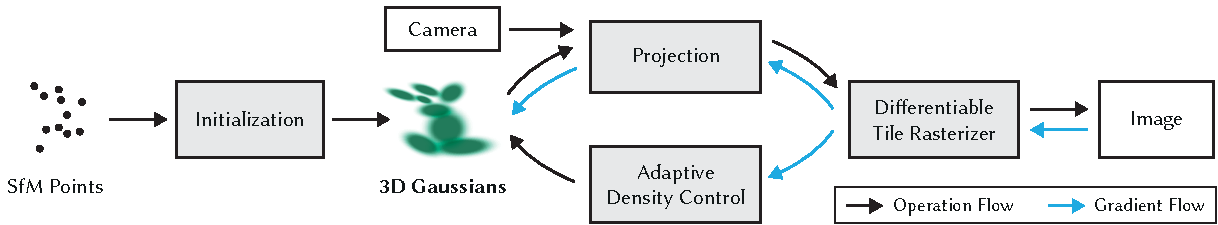
\includegraphics[width=\linewidth]{figures/overview/overview_01.pdf}
    \caption{
        Оптимизация начинается с разреженного облака точек SfM и создает набор 3D Гауссиан. Затем мы оптимизируем и адаптивно контролируем плотность этого набора Гауссиан. Во время оптимизации мы используем наш быстрый растеризатор на основе тайлов, что позволяет достичь конкурентного времени обучения по сравнению с самыми быстрыми современными методами радиусных полей. После обучения наш рендерер обеспечивает навигацию в реальном времени для широкого спектра сцен.
    }
    \label{fig:overview}
\end{figure*}
\section{Обзор}
Входными данными для нашего метода являются изображения статической сцены вместе с соответствующими камерами, откалиброванными с помощью SfM \cite{schoenberger2016sfm}, который в качестве побочного эффекта создает разреженное облако точек.
Из этих точек мы создаем набор 3D Гауссиан %
(Раздел~\ref{sec:3d-splats}), 
определяемых позицией (средним значением), матрицей ковариации и непрозрачностью $\alpha$, что позволяет использовать очень гибкий режим оптимизации. В результате получается достаточно компактное представление 3D сцены, отчасти потому, что высокоанизотропные объемные сплаты могут компактно представлять мелкие структуры. Направленная составляющая внешнего вида (цвет) радиусного поля представляется с помощью сферических гармоник (SH), что является стандартной практикой~\cite{plenoxels,mueller2022instant}. Наш алгоритм переходит к созданию представления радиусного поля (Раздел~\ref{sec:opt-dens}) через последовательность шагов оптимизации параметров 3D Гауссиан, то есть положения, ковариации, $\alpha$ и коэффициентов SH, чередующихся с операциями для адаптивного контроля плотности Гауссиан.
Ключом к эффективности нашего метода является наш растеризатор на основе тайлов (Раздел~\ref{sec:tile-raster}), который позволяет выполнять $\alpha$-смешивание анизотропных сплатов, учитывая порядок видимости благодаря быстрой сортировке. Наш быстрый растеризатор также включает быстрый обратный проход, отслеживая накопленные значения $\alpha$, без ограничения на количество Гауссиан, которые могут получать градиенты.
Обзор нашего метода представлен на Рис.~\ref{fig:overview}.
\section{Дифференцируемое 3D-сплаттинг Гауссиан}
\label{sec:3d-splats}

Наша цель — оптимизировать представление сцены, которое позволяет синтез высококачественных новых видов, начиная с разреженного набора (SfM) точек без нормалей. Для этого нам нужен примитив, который наследует свойства дифференцируемых объемных представлений, при этом оставаясь неструктурированным и явным для обеспечения очень быстрого рендеринга. Мы выбираем 3D Гауссианы, которые являются дифференцируемыми и могут быть легко спроецированы в 2D-сплаты, что позволяет быстро выполнять $\alpha$-смешивание для рендеринга.

Наше представление имеет сходства с предыдущими методами, использующими 2D-точки ~\cite{yifan19,kopanas21}, и предполагает, что каждая точка является маленьким плоским кругом с нормалью.
Учитывая крайнюю разреженность точек SfM, оценка нормалей крайне затруднена. Аналогично, оптимизация очень зашумленных нормалей из такой оценки также была бы очень сложной задачей.
Вместо этого мы моделируем геометрию как набор 3D Гауссиан, которые не требуют нормалей. Наши Гауссианы определяются полной 3D матрицей ковариации $\Sigma$, заданной в мировом пространстве~\cite{zwicker2001ewa} с центром в точке (среднее значение) $\mu$:
\begin{equation}
    G(x)~= e^{-\frac{1}{2}(x)^{T}\Sigma^{-1}(x)}
\end{equation}
\CORRECTION{где $|\Sigma|$ — это определитель $\Sigma$, являющейся симметричной матрицей размером 3$\times$3}{}. Этот Гауссиан умножается на $\alpha$ в нашем процессе смешивания.

Однако нам нужно спроецировать наши 3D Гауссианы в 2D для рендеринга.
Цвикер и др. ~\shortcite{zwicker2001ewa} демонстрируют, как выполнить эту проекцию в пространство изображения. Учитывая преобразование просмотра $W$,
матрица ковариации $\Sigma'$ в координатах камеры выглядит следующим образом:
\begin{equation}
    \label{eq:volume-render}
    \Sigma' = J W ~\Sigma ~W ^{T}J^{T}
\end{equation}
где $J$ — это якобиан аффинного приближения проективного преобразования. \CORRECTION{Авторы}{Цвикер и др. ~\shortcite{zwicker2001ewa}} также показывают, что если мы пропустим третью строку и столбец $\Sigma'$, 
мы получим матрицу дисперсии размером 2$\times$2 с той же структурой и свойствами, как если бы мы начинали с плоских точек с нормалями, как в предыдущих работах~\cite{kopanas21}.
    
Очевидный подход заключался бы в непосредственной оптимизации матрицы ковариации $\Sigma$ для получения 3D Гауссиан, представляющих радиусное поле. Однако матрицы ковариации имеют физический смысл только тогда, когда они являются положительно полуопределенными. 
Для нашей оптимизации всех параметров мы используем градиентный спуск, который сложно ограничить производством таких допустимых матриц, и шаги обновления и градиенты могут очень легко создавать недопустимые матрицы ковариации. 

В результате мы выбрали более интуитивное, но эквивалентно выразительное представление для оптимизации.
Матрица ковариации $\Sigma$ 3D Гауссиана аналогична описанию конфигурации эллипсоида.
Учитывая матрицу масштабирования $S$ и матрицу поворота $R$, мы можем найти соответствующую $\Sigma$:
\begin{equation}
    \Sigma = RSS^TR^T
\end{equation}

Чтобы позволить независимую оптимизацию обоих факторов, мы храним их отдельно: 3D вектор $s$ для масштабирования и кватернион $q$ для представления вращения. Их можно легко преобразовать в соответствующие матрицы и объединить, убедившись, что $q$ нормализован для получения единичного кватерниона.

Чтобы избежать значительных накладных расходов из-за автоматического дифференцирования во время обучения, мы явно выводим градиенты для всех параметров. Подробности точных вычислений производных находятся в приложении~\ref{sec:appa}.
\CORRECTION{Мы обсудим конкретный случай масштабирования и вращения (т.е., формы) 3D Гауссиан далее.}{}
\CORRECTION{Дифференцируемый рендерер выводит 
матрицу ковариации экранного пространства $\Sigma'$ размером $2\times2$.
Учитывая градиент потерь $\frac{dL}{d\Sigma'}$ %
(который мы считаем выходным сигналом дифференцируемого рендерера), 
мы можем применить цепное правило для вычисления градиентов и распространения потерь.}{}

Это представление анизотропной ковариации — подходящее для оптимизации — позволяет нам оптимизировать 3D Гауссианы для адаптации к геометрии различных форм в захваченных сценах, что приводит к довольно компактному представлению. 
Рис.~\ref{fig:aniso-cov} иллюстрирует такие случаи.
\begin{figure}[!h]
    \begin{overpic}[width=\columnwidth]{figures/anisotropic/real2}
        \put (61,3) {\color{white}Оригинал}
        \put (82.2,5) {\color{white}Сжатые} 
        \put (82,1.2) {\color{white}Гауссианы}
    \end{overpic}
    
    \caption{
        Мы визуализируем 3D Гауссианы после оптимизации, сжимая их на 60\% (справа). Это четко показывает анизотропные формы 3D Гауссиан, которые компактно представляют сложную геометрию после оптимизации. Слева — фактическое отрендеренное изображение.
    }
    \label{fig:aniso-cov}
\end{figure}
\section{Оптимизация с адаптивным контролем плотности 3D Гауссиан}
\label{sec:opt-dens}

Основой нашего подхода является шаг оптимизации, который создает плотный набор 3D Гауссиан, точно представляющих сцену для синтеза произвольных видов.
В дополнение к позициям $p$, $\alpha$ и ковариации $\Sigma$, мы также оптимизируем коэффициенты SH, представляющие цвет $c$ каждой Гауссианы, чтобы правильно захватывать зависимый от вида внешний вид сцены. 
Оптимизация этих параметров чередуется с шагами, контролирующими плотность Гауссиан для лучшего представления сцены.

\subsection{Оптимизация}

Оптимизация основана на последовательных итерациях рендеринга и сравнения полученного изображения с обучающими видами из захваченного набора данных. Неизбежно, геометрия может быть неправильно размещена из-за неоднозначностей проекции 3D в 2D. Таким образом, наша оптимизация должна уметь \emph{создавать} геометрию, а также \emph{уничтожать} или \emph{перемещать} геометрию, если она была неправильно расположена. Качество параметров ковариаций 3D Гауссиан критично для компактности представления, поскольку большие однородные области могут быть захвачены небольшим числом крупных анизотропных Гауссиан.

Мы используем методы стохастического градиентного спуска для оптимизации, полностью используя стандартные GPU-ускоренные фреймворки\TODO{ДОБАВИТЬ ссылку на pytorch}, и возможность добавлять пользовательские CUDA-ядра для некоторых операций, следуя современным рекомендациям~\cite{plenoxels,dvgo-cvpr2022}. В частности, наш быстрый растеризатор (см. Раздел~\ref{sec:tile-raster}) критичен для эффективности нашей оптимизации, поскольку это основное вычислительное узкое место оптимизации.

Мы используем сигмоидальную функцию активации для $\alpha$, чтобы ограничить её диапазоном $[0-1)$ и получить гладкие градиенты, и экспоненциальную функцию активации для масштаба ковариации по аналогичным причинам.

Мы оцениваем начальную ковариационную матрицу как изотропную Гауссиану с осями, равными среднему расстоянию до ближайших трех точек. 
Мы используем стандартную технику экспоненциального затухания, аналогичную Plenoxels~\cite{plenoxels}, но только для позиций. Функция потерь представляет собой комбинацию $\mathcal{L}_1$ и терма D-SSIM:

\begin{equation}
    \mathcal{L} = (1 - \lambda) \mathcal{L}_1 + \lambda \mathcal{L_{\textrm{D-SSIM}}}
\end{equation}

Мы используем $\lambda~=~0.2$ во всех наших тестах.
Подробнее о расписании обучения и других элементах представлено в Разделе~\ref{sec:impl}.

\subsection{Адаптивный контроль Гауссиан}

Мы начинаем с начального набора разреженных точек из SfM, а затем применяем наш метод для адаптивного контроля \REMOVAL{плотности \Dg~}\CORRECTION{количества 3D Гауссиан и их плотности на единицу объема}{числа Гауссиан и их плотности на единицу объема}\footnote{Плотность \CORRECTION{\Dg~}{Гауссиан} не следует путать, конечно же, с плотностью $\sigma$ в литературе NeRF.}, что позволяет нам перейти от начального разреженного набора Гауссиан к более плотному набору, который лучше представляет \CORRECTION{экран}{сцену} и имеет правильные параметры. 
После прогрева оптимизации (см. Раздел~\ref{sec:impl}), мы уплотняем каждые 100 итераций и удаляем любые Гауссианы, которые практически прозрачны, то есть с $\alpha$ меньше порога $\epsilon_{\alpha}$.

Наш адаптивный контроль \CORRECTION{плотности \Dg~}{Гауссиан} должен заполнять пустые области. Он фокусируется на областях с отсутствующими геометрическими особенностями («недостаточная реконструкция»), но также и в областях, где Гауссианы покрывают большие области сцены (что часто соответствует «чрезмерной реконструкции»).
\TODO{МОЖЕТ БЫТЬ ДОБАВИТЬ РИСУНОК (GK)}
Мы наблюдаем, что у обоих случаев есть \emph{большие} градиенты положения в пространстве видов.
Интуитивно это объясняется тем, что они соответствуют областям, которые еще не хорошо реконструированы, и оптимизация пытается переместить Гауссианы для исправления этого.

Поскольку оба случая являются хорошими кандидатами для уплотнения, \CORRECTION{следовательно}{} мы
уплотняем Гауссианы со средней величиной градиента положения в пространстве видов выше порога~$\tau_{\textrm{pos}}$, который мы установили равным $0.0002$ в наших тестах.

Далее мы представляем подробности этого процесса, проиллюстрированные на Рис.~\ref{fig:density_control}.

\begin{figure}[!h]
    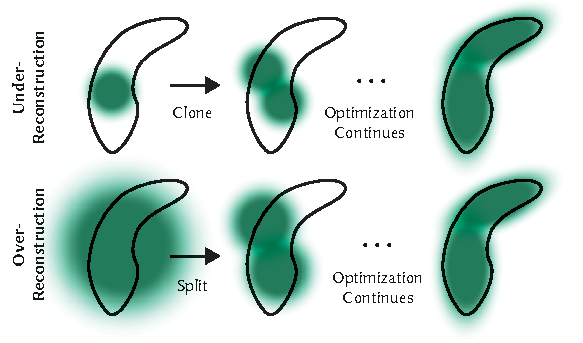
\includegraphics[width=\linewidth]{figures/density_control/density_control_01.pdf}
    \caption{
        \label{fig:density_control}
        Наша адаптивная схема уплотнения Гауссиан.
        \emph{Верхний ряд (недостаточная реконструкция)}: Когда мелкомасштабная геометрия (черный контур) недостаточно покрыта, мы клонируем соответствующую Гауссиану.
        \emph{Нижний ряд (чрезмерная реконструкция)}: Если мелкомасштабная геометрия представлена одним большим сплатом, мы разделяем его на два.
    }
\end{figure}

Для маленьких Гауссиан в недостаточно реконструированных регионах нам нужно покрыть новую геометрию, которая должна быть создана.
Для этого предпочтительно клонировать Гауссианы, просто создавая копию того же размера и перемещая её в направлении градиента положения.

С другой стороны, крупные Гауссианы в регионах с высокой дисперсией должны быть разделены на меньшие Гауссианы. Мы заменяем такие Гауссианы\REMOVAL{таким образом удаляем такие Гауссианы и вводим} двумя новыми\REMOVAL{Гауссианами}, и делим их масштаб на множитель $\phi~=~1.6$, который мы определили экспериментально.
Мы также инициализируем их положение, используя исходную 3D Гауссиану как PDF для выборки.

В первом случае мы обнаруживаем и лечим необходимость \CORRECTION{увеличения плотности \Dg}{увеличения как общего объема системы, так и количества Гауссиан}, тогда как во втором случае мы сохраняем \CORRECTION{общую плотность \Dg~ системы.}{общий объем, но увеличиваем количество Гауссиан.}
\CORRECTION{Учитывая, что наша задача не является строго выпуклой, оптимизация иногда может застрять в локальных минимумах, что может привести к необоснованному увеличению плотности Гауссиан.}{Подобно другим объемным представлениям, наша оптимизация может застрять с "плавающими" объектами близко к входным камерам; в нашем случае это может привести к необоснованному увеличению плотности Гауссиан.}
Эффективный способ умерить увеличение числа Гауссиан \CORRECTION{и справиться с плавающими объектами} — установить значение $\alpha$ близкое к нулю каждые $N=3000$ итераций. Затем оптимизация увеличивает $\alpha$ для Гауссиан, где это необходимо, позволяя нашему подходу удаления исключать Гауссианы с $\alpha$ меньше $\epsilon_{\alpha}$, как описано выше. \CORRECTION{Мы также}{Гауссианы могут сжиматься или расширяться и значительно пересекаться с другими, но мы периодически} удаляем \CORRECTION{}{Гауссианы, которые являются} очень большими \CORRECTION{Гауссианы} в мировом пространстве и \CORRECTION{Гауссианы}{те, что} имеют большой след в пространстве видов. Эта стратегия обеспечивает хорошее общее управление общим числом Гауссиан. \ADDITION{Гауссианы в нашей модели остаются примитивами в евклидовом пространстве в любое время; в отличие от других методов~\cite{barron2022mipnerf360,plenoxels}, нам не требуются стратегии уплотнения пространства, деформации или проекции для дальних или больших Гауссиан.}
\section{Быстрый дифференцируемый растеризатор для Гауссиан}
\label{sec:tile-raster}

Наши цели заключаются в обеспечении быстрого общего рендеринга и быстрой сортировки, чтобы позволить приближенное $\alpha$-смешивание — включая для анизотропных сплатов — и избежать жестких ограничений на количество сплатов, которые могут получать градиенты, как это существует в предыдущих работах~\cite{Lassner_2021_CVPR}.

Для достижения этих целей мы разработали тайловый растеризатор для Гауссиан, вдохновленный недавними подходами программного растеризатора~\cite{Lassner_2021_CVPR}, который позволяет предварительно сортировать примитивы для всего изображения сразу, избегая затрат на сортировку для каждого пикселя, что замедляло предыдущие решения с $\alpha$-смешиванием~\cite{kopanas21,kopanas22}. Наш быстрый растеризатор позволяет эффективно выполнять обратное распространение ошибки по произвольному числу смешанных Гауссиан с низким дополнительным потреблением памяти, требуя только постоянные накладные расходы на пиксель.
Наш конвейер растеризации полностью дифференцируем, и после проекции в 2D (Раздел~\ref{sec:3d-splats}) он может растеризовать анизотропные сплаты, аналогично предыдущим методам 2D сплаттинга~\cite{kopanas21}.

Наш метод начинается с разделения экрана на тайлы размером 16$\times$16, а затем переходит к отсечению 3D Гауссиан относительно пирамиды видимости и каждого тайла.
В частности, мы сохраняем только те Гауссианы, у которых интервал достоверности 99\% пересекает пирамиду видимости.
Кроме того, мы используем защитную полосу для тривиального отбраковывания Гауссиан в крайних положениях \ADDITION{(т.е., тех, чьи средние значения близки к ближней плоскости и сильно выходят за пределы пирамиды зрения)}, так как вычисление их проекции в 2D ковариацию было бы нестабильным.
Затем мы создаем экземпляры каждой Гауссианы в соответствии с количеством перекрываемых тайлов и присваиваем каждому экземпляру ключ, объединяющий глубину в пространстве просмотра и ID тайла. После этого мы сортируем Гауссианы на основе этих ключей, используя быструю GPU сортировку Radix~\cite{merrill2010revisiting}.
Обратите внимание, что здесь нет дополнительной сортировки точек на каждый пиксель, и смешивание выполняется на основе этой первоначальной сортировки. В результате, наше $\alpha$-смешивание может быть приближенным в некоторых конфигурациях.
Однако эти приближения становятся незначительными, когда \CORRECTION{точки}{сплаты} достигают размера отдельных пикселей.
Мы обнаружили, что этот выбор значительно повышает производительность обучения и рендеринга без создания заметных артефактов в сценах после сходимости.

После сортировки \CORRECTION{точек}{Гауссиан} мы формируем список для каждого тайла, определяя первый и последний элемент, отсортированный по глубине, который влияет на данный тайл. Для растеризации мы запускаем один блок потоков для каждого тайла. Каждый блок сначала совместно загружает пакеты \CORRECTION{точек}{Гауссиан} в разделяемую память, а затем, для данного пикселя, накапливает значения цвета и $\alpha$, проходя списки спереди назад, тем самым максимально увеличивая параллелизм как для загрузки/разделения данных, так и для их обработки.
Когда достигается целевое значение насыщения $\alpha$ в пикселе, соответствующий поток останавливается. С регулярными интервалами потоки в тайле проверяются, и обработка всего тайла завершается, когда все пиксели насыщаются (т.е., $\alpha$ становится равным 1). %
Детали сортировки и высокоуровневый обзор всего процесса растеризации представлены в Приложении~\ref{app:raster}.

Во время растеризации насыщение $\alpha$ является единственным критерием остановки. В отличие от предыдущих работ, мы не ограничиваем количество примитивов, участвующих в смешивании, которые получают обновления градиента. Мы применяем это свойство, чтобы позволить нашему подходу обрабатывать сцены с произвольной и изменяющейся глубиной сложности и точно обучать их, не прибегая к настройке гиперпараметров, специфичных для сцены.
Во время обратного прохода нам необходимо восстановить полную последовательность смешанных точек для каждого пикселя в прямом проходе. Одним из решений могло бы быть хранение произвольно длинных списков смешанных точек для каждого пикселя в глобальной памяти~\cite{kopanas21}. Чтобы избежать накладных расходов на динамическое управление памятью, мы выбираем повторное прохождение списков для каждого тайла; мы можем повторно использовать отсортированный массив Гауссиан и диапазоны тайлов из прямого прохода. Чтобы облегчить вычисление градиентов, мы теперь проходим их сзади наперёд.

Прохождение начинается с последней точки, которая оказала влияние на любой пиксель в тайле, и загрузка точек в разделяемую память снова происходит совместно. Кроме того, каждый пиксель будет проводить (дорогостоящее) тестирование наложения и обработку точек только если их \CORRECTION{индекс}{глубина} меньше или равна \CORRECTION{индексу}{глубине} последней точки, которая внесла вклад в его цвет во время прямого прохода.
Вычисление градиентов, описанных в Разделе~\ref{sec:3d-splats}, требует накопленных значений непрозрачности на каждом шаге во время исходного процесса смешивания.
\CORRECTION{Вместо хранения списка постепенно уменьшающихся значений непрозрачности во время прямого прохода, мы восстанавливаем эти значения из прямого прохода.}{Вместо обхода явного списка постепенно уменьшающихся значений непрозрачности в обратном проходе, мы можем восстановить эти промежуточные значения непрозрачности, сохраняя только общую накопленную непрозрачность в конце прямого прохода.}
В частности, каждая точка сохраняет окончательное накопленное значение непрозрачности $\alpha$ в прямом процессе; мы делим это на $\alpha$ каждой точки в нашем обратном проходе, чтобы получить необходимые коэффициенты для вычисления градиентов.
\section{Обсуждение результатов и оценка}
Мы обсудим некоторые детали реализации, представим результаты и проведем оценку нашего алгоритма в сравнении с предыдущими работами, а также проведем исследование по удалению компонентов.

\subsection{Реализация}
\label{sec:impl}
Мы реализовали наш метод на Python с использованием фреймворка PyTorch и написали пользовательские CUDA-ядра для растеризации, которые являются расширенными версиями предыдущих методов~\cite{kopanas21}, и используем библиотеку NVIDIA CUB для быстрой сортировки Radix sort~\cite{merrill2010revisiting}.
Также мы создали интерактивный просмотрщик, используя открытый исходный код SIBR~\cite{sibr2020}, который используется для интерактивного просмотра. \ADDITION{Мы использовали эту реализацию для измерения достигнутой частоты кадров}.
Исходный код и все наши данные доступны по адресу: \textcolor{blue}{\url{https://repo-sam.inria.fr/fungraph/3d-gaussian-splatting/}} 

\paragraph{Детали оптимизации}
Для стабильности мы «разогреваем» вычисления в более низком разрешении.
В частности, мы начинаем оптимизацию, используя изображения с разрешением в 4 раза ниже и увеличиваем их дважды после 250 и 500 итераций.
Оптимизация коэффициентов SH чувствительна к недостатку угловой информации. Для типичных «NeRF-like»
захватов, где центральный объект наблюдается с помощью фотографий, сделанных по всему полушарию вокруг него, оптимизация работает хорошо. Однако, если захват имеет пропущенные угловые области (например, при захвате угла сцены или выполнении «внутрь-наружу»~\cite{HRDB16} захвата), полностью некорректные значения для нулевого компонента SH (т.е., базового или диффузного цвета) могут быть получены в результате оптимизации.
Чтобы преодолеть эту проблему, мы начинаем с оптимизации только нулевого компонента, а затем вводим одну полосу SH после каждых 1000 итераций, пока все 4 полосы SH не будут представлены. %

\begin{table*}[!h]
    \caption{Оценка PSNR для тестовых прогонов. \ADDITION{Для этого эксперимента мы вручную понизили разрешение высококачественных версий входных изображений каждой сцены до установленного разрешения рендеринга наших других экспериментов. Это снижает случайные артефакты (например, из-за сжатия JPEG в предварительно уменьшенных входных данных Mip-NeRF360).}}
    \centering
    \begin{tabular}{l|ccc|ccc|cc}
        ~ & Truck-5K & Garden-5K & Bicycle-5K & Truck-30K & Garden-30K & Bicycle-30K & Average-5K & Average-30K \\ \hline
        Limited-BW  & 14.66 & 22.07 & 20.77 & 13.84 & 22.88 & 20.87 & 19.16 & 19.19 \\
        Random Init & 16.75 & 20.90 & 19.86 & 18.02 & 22.19 & 21.05 & 19.17 & 20.42 \\ 
        No-Split    & 18.31 & 23.98 & 22.21 & 20.59 & 26.11 & 25.02 & 21.50 & 23.90 \\ 
        No-SH       & \cellcolor{yellow!40}22.36 & 25.22 & \cellcolor{orange!40}22.88 & \cellcolor{yellow!40}24.39 & 26.59 & \cellcolor{yellow!40}25.08 & \cellcolor{yellow!40}23.48 & \cellcolor{yellow!40}25.35 \\ 
        No-Clone    & 22.29 & \cellcolor{orange!40}25.61 & 22.15 & \cellcolor{red!40}24.82 & \cellcolor{orange!40}27.47 & \cellcolor{orange!40}25.46 & 23.35 & \cellcolor{orange!40}25.91 \\  
        Isotropic   & \cellcolor{orange!40}22.40 & \cellcolor{yellow!40}25.49 & \cellcolor{yellow!40}22.81 & 23.89 & \cellcolor{yellow!40}27.00 & 24.81 & \cellcolor{orange!40}23.56 & 25.23 \\  
        Full        & \cellcolor{red!40}22.71 & \cellcolor{red!40}25.82 & \cellcolor{red!40}23.18 & \cellcolor{orange!40}24.81 &\cellcolor{red!40} 27.70 & \cellcolor{red!40}25.65 & \cellcolor{red!40}23.90 & \cellcolor{red!40}26.05 \\  
    \end{tabular}
    \label{tab:ablation_table}
\end{table*}

\subsection{Результаты и оценка}
\paragraph{Результаты.}
Мы протестировали наш алгоритм на общем количестве \CORRECTION{11}{13} реальных сцен, взятых из ранее опубликованных наборов данных и синтетического набора данных Blender ~\cite{mildenhall2020nerf}. 
В частности, мы протестировали наш подход на полном наборе сцен, представленных в Mip-Nerf360~\cite{barron2022mipnerf360}, который является текущим уровнем качества рендеринга NeRF, двух сценах из набора данных Tanks\&Temples \shortcite{knapitsch2017tanks} и двух сценах, предоставленных Hedman et al.~\cite{hedman2018deep}. 
Сцены, которые мы выбрали, имеют очень разные стили захвата, и охватывают как ограниченные внутренние сцены, так и большие неограниченные внешние среды.
\CORRECTION{Мы используем одинаковые значения параметров для всех наших запусков, за исключением скорости обучения для ковариации: для всех сцен она составляет 0.001, за исключением \textsc{Train}, \textsc{DrJohnson} и \textsc{Playroom} (см. Рис.~\mbox{\ref{fig:comparisons}}), где она делится на три, поскольку стиль захвата намного менее структурирован.}{Мы используем ту же конфигурацию гиперпараметров для всех экспериментов в нашей оценке.} Все результаты указаны для работы на GPU A6000\ADDITION{, за исключением метода Mip-NeRF360 (см. ниже)}.
В дополнительных материалах мы показываем видео пути рендеринга для выбора сцен, содержащих виды, далекие от входных фотографий.

\paragraph{Реальные сцены.}
В плане качества текущий уровень развития — это Mip-Nerf360~\cite{barron2021mipnerf}. Мы сравниваемся с этим методом как с качественным эталоном. Мы также сравниваемся с двумя самыми последними быстрыми методами NeRF: InstantNGP~\cite{mueller2022instant} и Plenoxels~\cite{plenoxels}.
Мы используем разделение train/test для наборов данных, используя методологию, предложенную Mip-NeRF360, беря каждую 8-ю фотографию для теста, для последовательных и значимых сравнений для генерации метрик ошибок, используя стандартные метрики PSNR, L-PIPS и SSIM, наиболее часто используемые в литературе; пожалуйста, см. \CORRECTION{Таб.}{Таблица}~\ref{tab:comparisons}. \CORRECTION{Обратите внимание, что мы запустили улучшенную версию кода Mip-NeRF360, которая дает немного лучшие числа, чем в оригинальной публикации.}{Все числа в таблице взяты из наших собственных запусков кода авторов для всех предыдущих методов, за исключением тех, что относятся к Mip-NeRF360 на их наборе данных, где мы скопировали числа из оригинальной публикации, чтобы избежать путаницы о текущем уровне развития. Для изображений в наших
фигурах мы использовали наш собственный запуск Mip-NeRF360: числа для этих запусков находятся в Приложении~\ref{sec:appd}.}
Мы также показываем среднее время обучения, скорость рендеринга и объем памяти, используемый для хранения оптимизированных параметров. Мы сообщаем результаты для базовой конфигурации InstantNGP (Base), которая работает в течение 35K итераций, а также немного большей сети, предложенной авторами (Big), и двух конфигураций, 7K и 30K итераций для нашего метода. 
Мы показываем разницу в визуальном качестве для наших двух конфигураций на Рис.~\ref{fig:5vs40min}. Во многих случаях качество после 7K итераций уже довольно хорошее.
Время обучения различается в зависимости от наборов данных, и мы сообщаем их отдельно. Обратите внимание, что разрешение изображений также различается в зависимости от наборов данных.
В \CORRECTION{дополнительных материалах}{проектном сайте} мы предоставляем все рендеры тестовых видов, которые мы использовали для вычисления статистики для всех методов (наших и предыдущих работ) на \CORRECTION{\textsc{bicycle}, \textsc{Truck} и \textsc{Playroom}}{все сцены.} Обратите внимание, что мы сохранили исходное входное разрешение для всех рендеров.
Таблица показывает, что наша полностью сходившаяся модель достигает качества наравне и иногда немного лучше, чем у лидирующего метода Mip-NeRF360; обратите внимание, что на том же оборудовании их среднее время обучения составило 48 часов\footnote{Мы обучали Mip-NeRF360 на узле с 4 GPU A100 в течение 12 часов, что эквивалентно 48 часам на одном GPU. Обратите внимание, что A100 быстрее, чем GPU A6000.}, по сравнению с нашими 35-45 минутами, а их время рендеринга составляет 10 секунд/кадр. Мы достигаем сравнимого качества с InstantNGP и Plenoxels после 5-10 минут обучения, но дополнительное время обучения позволяет нам достичь уровня современного развития, чего нельзя сказать о других быстрых методах. Для Tanks \& Temples мы достигаем аналогичного качества как базовый InstantNGP при аналогичном времени обучения ($\sim$\CORRECTION{8}{7} минут в нашем случае).
Мы также показываем визуальные результаты этого сравнения для тестового вида для нашего метода и предыдущих методов рендеринга, выбранных для сравнения, на Рис.~\ref{fig:comparisons}; результаты нашего метода после 30K итераций обучения. Мы видим, что в некоторых случаях даже Mip-NeRF360 имеет оставшиеся артефакты, которых избегает наш метод (например, размытость в растительности — в \textsc{Bicycle, Stump} — или на стенах в \textsc{Room}).
В дополнительном видео и на веб-странице мы предоставляем сравнения путей с расстояния. Наш метод сохраняет визуальные детали хорошо покрытых областей даже с дальнего расстояния, чего не всегда можно добиться другими методами.

\paragraph{Синтетические ограниченные сцены}
Помимо реалистичных сцен, мы также оцениваем наш подход на синтетическом наборе данных \emph{Blender} \cite{mildenhall2020nerf}. Сцены в вопросе предоставляют исчерпывающий набор видов, ограничены в размере и предоставляют точные параметры камеры. В таких сценариях мы можем достичь результатов уровня современного состояния даже с произвольной инициализацией: мы начинаем обучение с 100K равномерно случайных Гауссиан внутри объема, охватывающего границы сцены. Наш подход быстро и автоматически сокращает их до примерно 6--10K значимых Гауссиан. Конечный размер обученной модели после 30K итераций достигает около 200--500K Гауссиан на сцену. Мы сообщаем и сравниваем наши достигнутые значения PSNR с предыдущими методами в \CORRECTION{Таб.}{Таблица}~\ref{tab:results_synthetic} с использованием белого фона для совместимости. Примеры можно увидеть на Рис.~\ref{fig:ablation-aniso} (второе изображение слева) и в дополнительных материалах. \ADDITION{Обученные синтетические сцены рендерятся со скоростью 180--300 FPS.}

\paragraph{Компактность}
В сравнении с предыдущими явными представлениями сцен, анизотропные Гауссианы, используемые в нашей оптимизации, способны моделировать сложные формы с меньшим количеством параметров.
Мы демонстрируем это, оценивая наш подход против высоко компактных, основанных на точках моделей, полученных \cite{zhang2022}.
Мы начинаем с их начального облака точек, которое получено путем пространственного вырезания с масками переднего плана %
и оптимизируем, пока не достигнем равенства с их заявленными значениями PSNR. Обычно это происходит в течение 2--4 минут. Мы превышаем их заявленные метрики, используя примерно четверть их количества точек, что приводит к среднему размеру модели 3.8 МБ, по сравнению с их 9 МБ. Мы отмечаем, что для этого эксперимента мы использовали только две степени наших сферических гармоник, аналогично их подходу.

\subsection{Исследования по удалению компонентов}
\label{sec:ablations}
Мы выделили различные вклады и алгоритмические решения, которые мы приняли, и создали серию экспериментов для измерения их влияния. В частности, мы тестируем следующие аспекты нашего алгоритма: инициализация из SfM, наши стратегии уплотнения, анизотропная ковариация, тот факт, что мы позволяем неограниченному количеству сплатов иметь градиенты
и использование сферических гармоник.
Количественное влияние каждого выбора суммировано в \CORRECTION{Таб.}{Таблица}~\ref{tab:ablation_table}.

\begin{figure}[!h]
    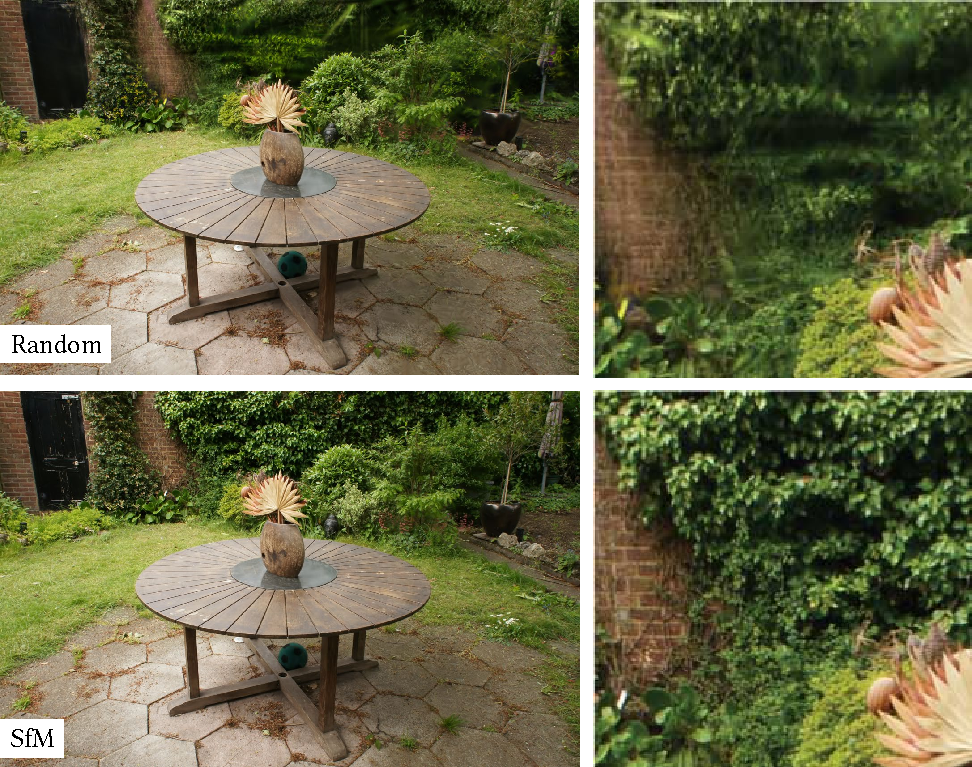
\includegraphics[width=\linewidth]{figures/ablations/random_vs_sfm2.pdf}
    \caption{
        \label{fig:random}
        Инициализация с точками SfM помогает. Выше: инициализация с случайным облаком точек. Ниже: инициализация с использованием точек SfM.
    }
\end{figure}

\paragraph{Инициализация из SfM}
Мы также оцениваем важность инициализации 3D Гауссиан из облака точек SfM.
Для этого исследования мы равномерно выбираем куб с размером, равным трем размерам ограничивающего прямоугольника входных камер. Мы наблюдаем, что наш метод работает относительно хорошо, избегая полного провала даже без точек SfM. Вместо этого он ухудшается в основном на заднем плане, см. Рис.~\ref{fig:random}. Также в областях, плохо покрытых обучающими видами, метод случайной инициализации кажется более подверженным наличию "плавающих" точек, которые не могут быть удалены оптимизацией. С другой стороны, синтетический набор данных NeRF не проявляет такого поведения, потому что у него нет заднего плана и он хорошо ограничен входными камерами (см. обсуждение выше).

\begin{figure}[!h]
    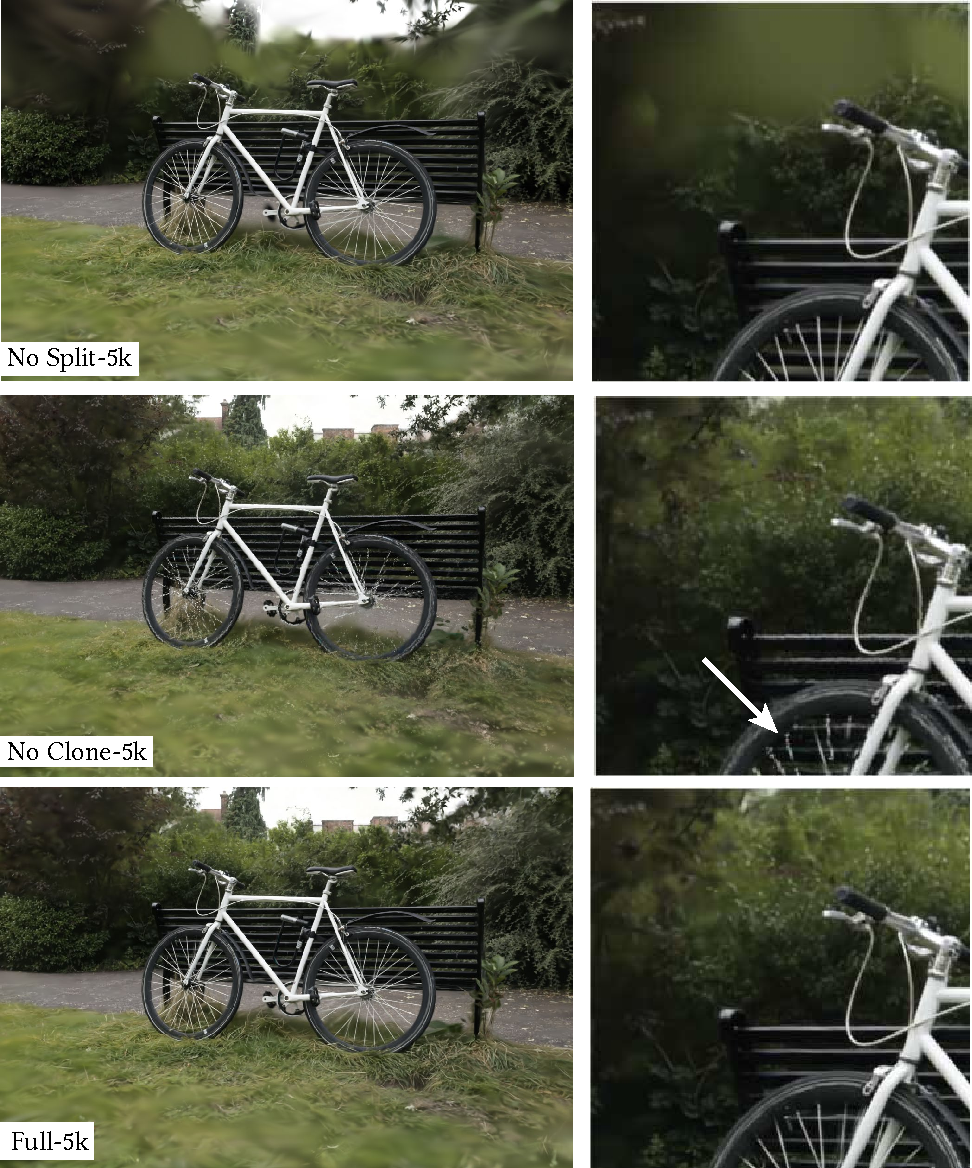
\includegraphics[width=\linewidth]{figures/ablations/densification.pdf}
    \caption{
        \label{fig:densification_ablate}
        Исследование стратегии уплотнения для двух случаев "клонирование" и "разделение" (Раздел~\ref{sec:opt-dens}).
    }
\end{figure}

\paragraph{Уплотнение.}
Мы далее оцениваем наши два метода уплотнения, а именно стратегию клонирования и разделения, описанные в Разделе~\ref{sec:opt-dens}. Мы отключаем каждый метод по отдельности и оптимизируем, используя остальную часть метода без изменений. Результаты показывают, что разделение больших Гауссиан важно для обеспечения хорошей реконструкции заднего плана, как видно на Рис.~\ref{fig:densification_ablate}, тогда как клонирование маленьких Гауссиан вместо их разделения позволяет достичь лучшей и более быстрой сходимости, особенно когда в сцене появляются тонкие структуры.

\begin{figure}[!h]
    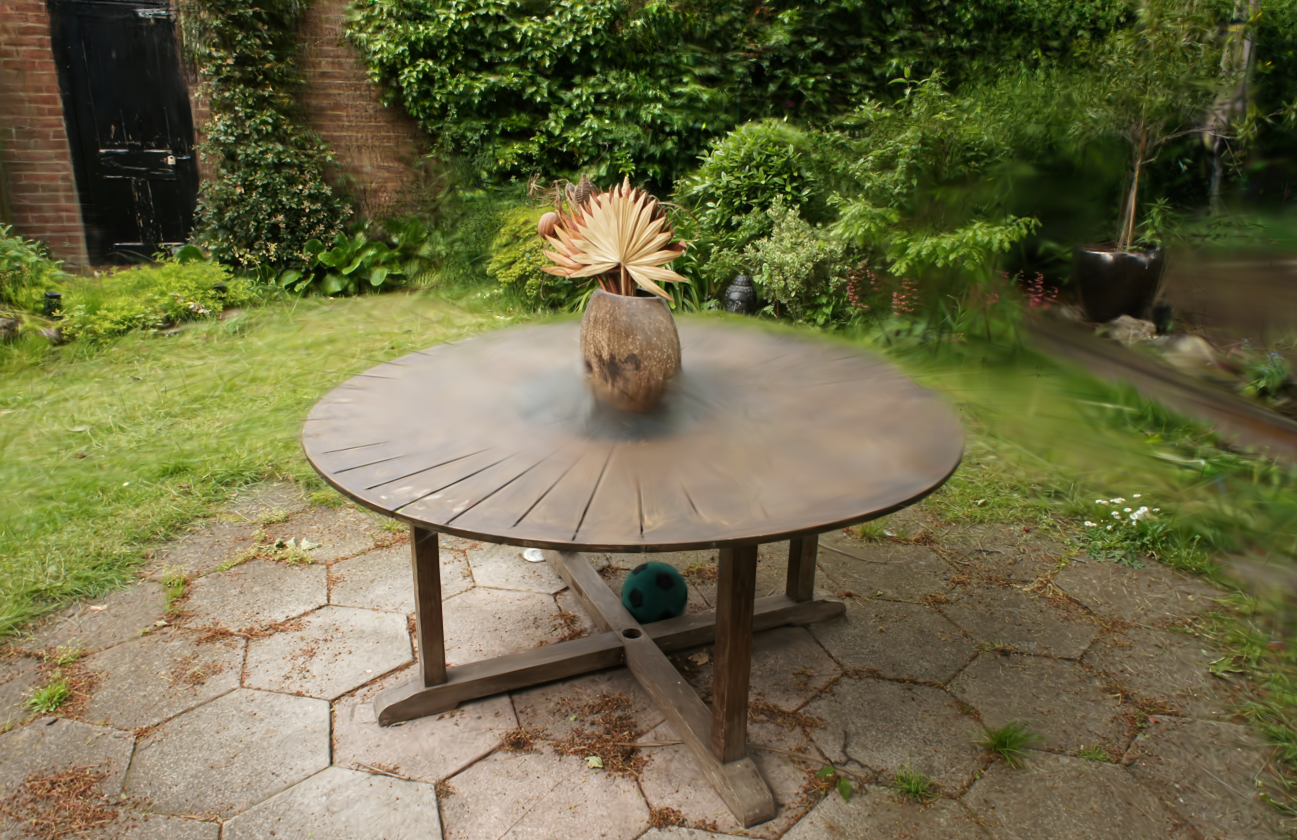
\includegraphics[width=.49\linewidth]{figures/ablations/images/30k/garden/limitedBW.png}
    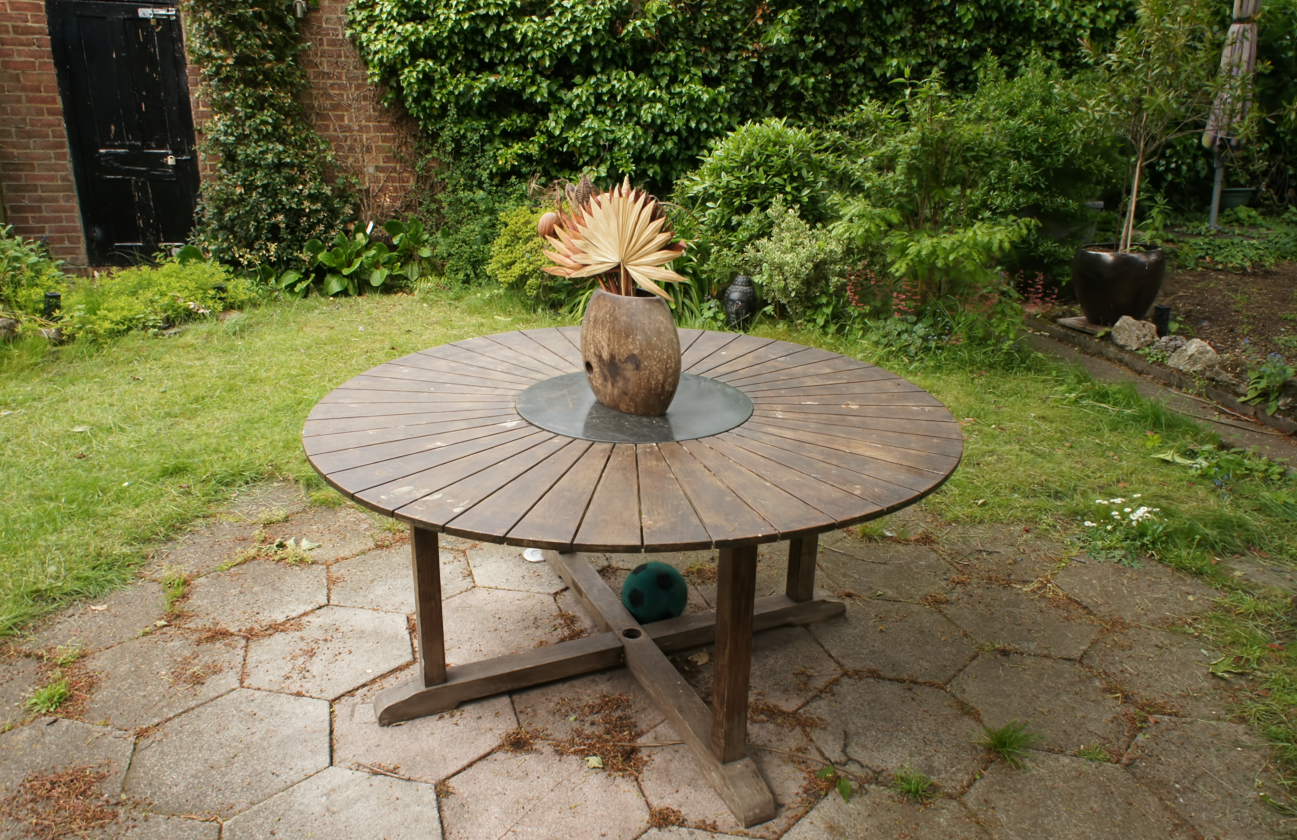
\includegraphics[width=.49\linewidth]{figures/ablations/images/30k/garden/full.png}
    \caption{
        Если мы ограничим количество точек, получающих градиенты, эффект на визуальное качество будет значительным.
        Слева: лимит в 10 Гауссиан, получающих градиенты. Справа: наш полный метод.
        \label{fig:gradients}
    }
\end{figure}

\paragraph{Неограниченная глубина сложности сплатов с градиентами.}
Мы оцениваем, даст ли пропуск вычисления градиентов после $N$ передних точек нам скорость без ущерба для качества, как предложено в Pulsar~\cite{Lassner_2021_CVPR}. В этом тесте мы выбираем N=10, что в два раза больше значения по умолчанию в Pulsar, но это привело к нестабильной оптимизации из-за серьезного приближения в вычислении градиентов. Для сцены \textsc{Truck} качество ухудшилось на 11 дБ в PSNR (см. \CORRECTION{Таб.}{Таблица}~\ref{tab:ablation_table}, Limited-BW), и визуальный результат показан на Рис.~\ref{fig:gradients} для \textsc{Garden}.

\paragraph{Анизотропная ковариация.}
Важным алгоритмическим выбором в нашем методе является оптимизация полной матрицы ковариации для 3D Гауссиан. Чтобы продемонстрировать влияние этого выбора, мы проводим исследование, где удаляем анизотропию, оптимизируя одно скалярное значение, которое управляет радиусом 3D Гауссиана по всем трем осям. Результаты этой оптимизации представлены визуально на Рис.~\ref{fig:ablation-aniso}. Мы наблюдаем, что анизотропия значительно улучшает способность 3D Гауссиан выравниваться с поверхностями, что, в свою очередь, позволяет достичь гораздо более высокого качества рендеринга, сохраняя то же количество точек.

\begin{figure*}[!h]
    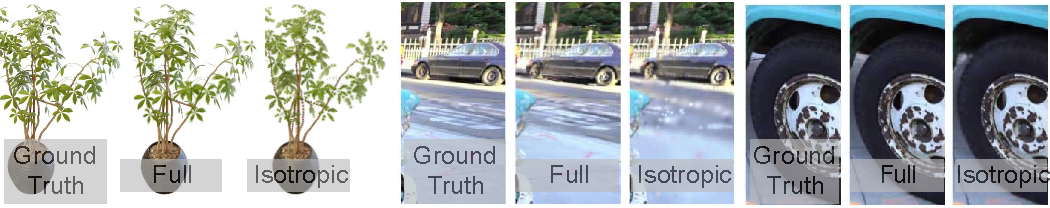
\includegraphics{figures/ablations/isotropy_vs_anisotropy2.pdf}
    \caption{
        \label{fig:ablation-aniso}
        Мы обучаем сцены с отключенной и включенной анизотропией Гауссиан. Использование анизотропных объемных сплатов позволяет моделировать мелкие структуры и оказывает значительное влияние на визуальное качество. Обратите внимание, что в иллюстративных целях мы ограничили \textsc{Ficus} использованием не более 5K Гауссиан в обеих конфигурациях.
    }
\end{figure*}

\paragraph{Сферические гармоники.}
Наконец, использование сферических гармоник улучшает наши общие показатели PSNR, поскольку они компенсируют зависимые от вида эффекты (\CORRECTION{Таб.}{Таблица}~\ref{tab:ablation_table}).

\subsection{Ограничения}
Наш метод не без ограничений.
В регионах, где сцена плохо наблюдаема, у нас есть артефакты; в таких регионах другие методы также сталкиваются с трудностями (например, Mip-NeRF360 на Рис.~\ref{fig:limit}). 
Хотя анизотропные Гауссианы имеют много преимуществ, как описано выше,
наш метод может создавать вытянутые артефакты или «пятнистые» Гауссианы (см. Рис.~\ref{fig:limit-under}); снова предыдущие методы также испытывают трудности в этих случаях.
У нас также иногда возникают скачкообразные артефакты, когда наша оптимизация создает большие Гауссианы; это обычно происходит в областях с зависимым от вида внешним видом.
Одной из причин этих скачкообразных артефактов является тривиальное отклонение Гауссиан через защитную полосу в растеризаторе. Более принципиальный подход к отбраковке мог бы уменьшить эти артефакты. \ADDITION{Другим фактором является наш простой алгоритм видимости, который может приводить к тому, что Гауссианы внезапно меняют порядок глубины/смешивания. Этого можно было бы избежать с помощью сглаживания, что мы оставляем для будущей работы.}
Кроме того, в настоящее время мы не применяем никакой регуляризации к нашей оптимизации; это помогло бы как с невидимыми областями, так и с скачкообразными артефактами.
\ADDITION{Хотя мы использовали одни и те же гиперпараметры для всей оценки, ранние эксперименты показывают, что уменьшение скорости обучения положения может быть необходимо для сходимости в очень больших сценах (например, городских наборах данных).}
Хотя мы весьма компактны по сравнению с предыдущими точечными подходами, потребление нашей памяти значительно выше, чем у решений на основе NeRF. \ADDITION{Во время обучения больших сцен пиковое потребление GPU-памяти может превышать 20 ГБ в нашей неоптимизированной прототипе. Однако эта цифра могла бы быть значительно снижена за счет тщательной низкоуровневой реализации логики оптимизации (аналогично InstantNGP). Рендеринг обученной сцены требует достаточного объема GPU-памяти для хранения полной модели (несколько сотен мегабайт для крупных сцен) и дополнительных 30--500 МБ для растеризатора, в зависимости от размера сцены и разрешения изображения. Мы отмечаем, что есть множество возможностей для дальнейшего снижения потребления памяти нашим методом.} Техники сжатия для облаков точек — это хорошо изученная область~\cite{de2016compression}; было бы интересно увидеть, как такие подходы могут быть адаптированы к нашему представлению.

\begin{figure}[!h]
    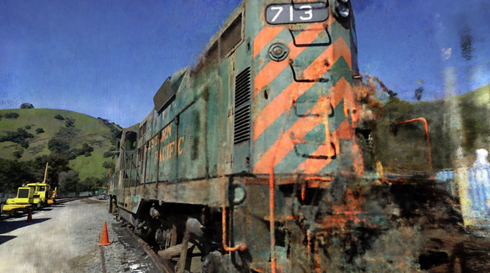
\includegraphics[width=0.49\columnwidth]{results/limitations/color_009_s.png}
    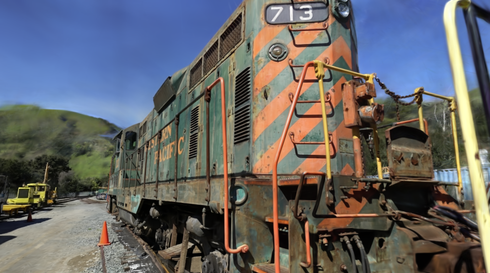
\includegraphics[width=0.49\columnwidth]{results/limitations/00073_s.png}
    \caption{
        \label{fig:limit}
        Сравнение артефактов сбоя: Mip-NeRF360 имеет «плавающие объекты» и зернистую текстуру (слева, передний план), тогда как наш метод производит грубые, анизотропные Гауссианы, приводящие к низкой детализации (справа, задний план). Сцена \textsc{Train}.
    }
\end{figure}

\begin{figure}[!h]
    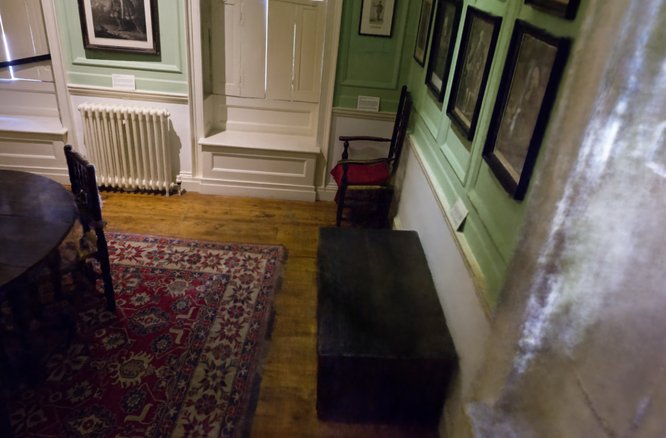
\includegraphics[width=0.49\linewidth]{figures/extremeviews/color_032_s.png}
    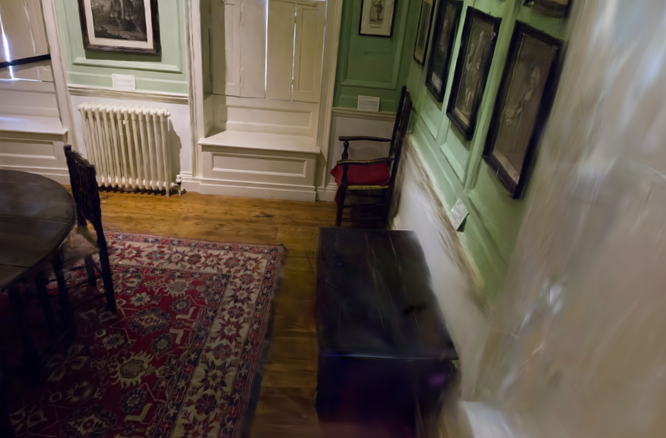
\includegraphics[width=0.49\linewidth]{figures/extremeviews/IMG_6589_s.png}
    \caption{
        В видах, которые мало пересекаются с теми, что были видны во время обучения, наш метод может производить артефакты (справа). Опять же, Mip-NeRF360 также имеет артефакты в этих случаях (слева). Сцена \textsc{DrJohnson}.
        \label{fig:limit-under}
    }
\end{figure}
\section{Обсуждение и выводы}

Мы представили первый подход, который действительно позволяет рендеринг радиусных полей в реальном времени с высоким качеством в широком диапазоне сцен и стилей захвата, требуя при этом времени обучения, конкурентного с самыми быстрыми предыдущими методами.

Наш выбор примитива 3D Гауссиан сохраняет свойства объемного рендеринга для оптимизации, одновременно позволяя непосредственно выполнять быстрое растеризованное сплатирование. Наша работа демонстрирует, что — вопреки широко распространенному мнению — непрерывное представление \emph{не} является строго необходимым для обеспечения быстрого и высококачественного обучения радиусных полей.

Большая часть ($\sim$80\%) нашего времени обучения тратится на код Python, поскольку мы создали наше решение на PyTorch, чтобы позволить другим легко использовать наш метод. Только растеризация реализована как оптимизированные CUDA ядра. Мы ожидаем, что перенос всей оптимизации целиком на CUDA, как это сделано, например, в InstantNGP~\cite{mueller2022instant}, может обеспечить значительное дальнейшее ускорение для приложений, где производительность имеет ключевое значение.

Мы также продемонстрировали важность построения на принципах рендеринга в реальном времени, используя мощь GPU и скорость архитектуры программного конвейера растеризации. Эти проектные решения являются ключом к производительности как для обучения, так и для рендеринга в реальном времени, предоставляя конкурентное преимущество в производительности над предыдущим объемным трассированием лучей.

Было бы интересно выяснить, можно ли использовать наши Гауссианы для выполнения реконструкции сетки захваченной сцены. Помимо практических последствий, учитывая широкое использование сеток, это позволило бы нам лучше понять, где именно находится наш метод в континууме между объемными и поверхностными представлениями.

Подводя итог, мы представили первое решение для рендеринга радиусных полей в реальном времени с качеством рендеринга, соответствующим лучшим дорогим предыдущим методам, и временем обучения, конкурентным с самыми быстрыми существующими решениями.

\begin{acks}
Это исследование было профинансировано грантом ERC Advanced FUNGRAPH № 788065 \textcolor{blue}{\url{http://fungraph.inria.fr}}. Авторы благодарны Adobe за щедрые пожертвования, инфраструктуру OPAL от Université Côte d’Azur и за ресурсы HPC от GENCI–IDRIS (Грант 2022-AD011013409). Авторы благодарят анонимных рецензентов за ценные отзывы, П.\ Хедмана и А.\ Тевари за проверку ранних черновиков, а также Т.\ Мюллера, А.\ Ю и С.\ Фридович-Кейла за помощь в сравнениях. 
\end{acks}

\bibliographystyle{ACM-Reference-Format}
\bibliography{points.bib}

\begin{appendix}
    \section{Подробности вычисления градиентов}
    \label{sec:appa}
    Напомним, что $\Sigma$/$\Sigma'$ — это матрицы ковариации Гауссиан в мировом/видовом пространстве, $q$ — это вращение, а $s$ — масштабирование, $W$ — это преобразование просмотра, а $J$ — Якобиан аффинного приближения проективного преобразования.
    Мы можем применить цепное правило для нахождения производных по масштабированию и вращению:
    \begin{equation}
        \frac{d\Sigma'}{ds} = \frac{d\Sigma'}{d\Sigma}\frac{d\Sigma}{ds}
    \end{equation}
    и 
    \begin{equation}
        \frac{d\Sigma'}{dq} = \frac{d\Sigma'}{d\Sigma}\frac{d\Sigma}{dq}
    \end{equation}
    Упростив уравнение~\ref{eq:volume-render}, используя $U = JW$ и $\Sigma'$ как (симметричную) верхнюю левую $2\times2$ матрицу $U \Sigma U^T$, обозначая элементы матрицы индексами, мы можем найти частные производные
    $
        \frac{\partial \Sigma'}{\partial \Sigma_{ij}} = \left(\begin{smallmatrix}
            U_{1,i}U_{1,j} & U_{1,i} U_{2,j}\\
            U_{1,j} U_{2,i} & U_{2,i}U_{2,j}
        \end{smallmatrix}\right)
    $.
    Далее ищем производные $\frac{d\Sigma}{ds}$ и $\frac{d\Sigma}{dq}$. Поскольку $\Sigma = RSS^TR^T$, мы можем вычислить $M = RS$ и переписать $\Sigma = MM^T$. Таким образом, мы можем записать $\frac{d\Sigma}{ds} = \frac{d\Sigma}{dM} \frac{dM}{ds}$ и $\frac{d\Sigma}{dq} = \frac{d\Sigma}{dM} \frac{dM}{dq}$. Так как матрица ковариации $\Sigma$ (и её градиент) симметрична, общая первая часть компактно находится как $\frac{d\Sigma}{dM} = 2M^T$. Для масштабирования также имеем
    $	\frac{\partial M_{i,j}}{\partial s_k} =  \left\{\begin{array}{lr}
        R_{i,k} & \text{если j = k}\\
        0 & \text{иначе}
    \end{array}\right\}$.
    Чтобы вывести градиенты для вращения, вспомним преобразование единичного кватерниона $q$ с действительной частью $q_r$ и мнимыми частями $q_i, q_j, q_k$ в матрицу вращения $R$:
    \begin{equation}
        R(q) = 2\begin{pmatrix}
            \frac{1}{2} - (q_j^2 + q_k^2) & (q_i q_j - q_r q_k) & (q_i q_k + q_r q_j)\\
            (q_i q_j + q_r q_k) & \frac{1}{2} - (q_i^2 + q_k^2) & (q_j q_k - q_r q_i)\\
            (q_i q_k - q_r q_j) & (q_j q_k + q_r q_i) & \frac{1}{2} - (q_i^2 + q_j^2)
        \end{pmatrix}
        \label{eq:quat}
    \end{equation}
    В результате получаем следующие градиенты для компонентов $q$:
    \begin{equation}
        \begin{aligned}
            &\frac{\partial M}{\partial q_r} = 2 \left(\begin{smallmatrix}
                0 & -s_y q_k & s_z q_j\\
                s_x q_k & 0 & -s_z q_i\\
                -s_x q_j & s_y q_i & 0
            \end{smallmatrix}\right), 
            &\frac{\partial M}{\partial q_i} = 2\left(\begin{smallmatrix}
                0 & s_y q_j & s_z q_k\\
                s_x q_j & -2 s_y q_i & -s_z q_r\\
                s_x q_k & s_y q_r & -2 s_z q_i
            \end{smallmatrix}\right)
            \\
            &\frac{\partial M}{\partial q_j} = 2\left(\begin{smallmatrix}
                -2 s_x q_j & s_y q_i & s_z q_r\\
                s_x q_i & 0 & s_z q_k\\
                -s_x q_r & s_y q_k & -2s_z q_j
            \end{smallmatrix}\right),
            &\frac{\partial M}{\partial q_k} = 2\left(\begin{smallmatrix}
                -2 s_x q_k & -s_y q_r & s_z q_i\\
                s_x q_r & -2s_y q_k & s_z q_j\\
                s_x q_i & s_y q_j & 0
            \end{smallmatrix}\right)
        \end{aligned}
    \end{equation} 
Вывод градиентов для нормализации кватерниона тривиален.
    \section{Алгоритм оптимизации и увеличения плотности}
    Наши алгоритмы оптимизации и увеличения плотности суммированы в Алгоритме \ref{alg:optimization}.
    \begin{algorithm}[!h]
        \caption{Оптимизация и увеличение плотности\\
        $w$, $h$: ширина и высота обучающих изображений}
        \label{alg:optimization}
        \begin{algorithmic}
            \State $M \gets$ SfM Точки	\Comment{Позиции}
            \State $S, C, A \gets$ InitAttributes() \Comment{Ковариации, Цвета, Непрозрачности}
            \State $i \gets 0$	\Comment{Счетчик итераций}
            \While{не сходится}
            \State $V, \hat{I} \gets$ SampleTrainingView()	\Comment{Камера $V$ и Изображение}
            \State $I \gets$ Растеризовать($M$, $S$, $C$, $A$, $V$)	\Comment{Алг.~\ref{alg:rasterize}}
            \State $L \gets Loss(I, \hat{I}) $ \Comment{Потери}
            \State $M$, $S$, $C$, $A$ $\gets$ Adam($
abla L$) \Comment{Обратное распространение ошибки и шаг}
            \If{IsRefinementIteration($i$)}
            \ForAll{Гауссианы $(\mu, \Sigma, c, \alpha)$ $\textbf{в}$ $(M, S, C, A)$}
            \If{$\alpha < \epsilon$ или IsTooLarge($\mu, \Sigma)$}	\Comment{Обрезка}
            \State УдалитьГауссиану()	
            \EndIf
            \If{$
abla_p L > \tau_p$} \Comment{Увеличение плотности}
            \If{$\|S\| > \tau_S$}	\Comment{Пересоздание}
            \State РазделитьГауссиану($\mu, \Sigma, c, \alpha$)
            \Else								\Comment{Недостаточная реконструкция}
            \State КлонироватьГауссиану($\mu, \Sigma, c, \alpha$)
            \EndIf	
            \EndIf
            \EndFor		
            \EndIf
            \State $i \gets i+1$
            \EndWhile
        \end{algorithmic}
    \end{algorithm}
    \section{Подробности растеризатора}
    \label{app:raster}
    \paragraph{Сортировка.}
    Наш дизайн основан на предположении о большом количестве маленьких сплатов, и мы оптимизируем это путем однократной сортировки сплатов для каждого кадра с использованием поразрядной сортировки в начале.
    Мы разделяем экран на тайлы размером 16x16 пикселей (или бины). Мы создаем список сплатов для каждого тайла, создавая экземпляр каждого сплата в каждом перекрывающем его тайле 16$\times$16. Это приводит к умеренному увеличению числа Гауссиан для обработки, 
    что, однако, амортизируется более простым потоком управления и высокой параллельностью оптимизированной поразрядной сортировки GPU~\cite{merrill2010revisiting}.
    Мы назначаем ключ для каждого экземпляра сплата длиной до 64 бит, где младшие 32 бита кодируют его проекционную глубину, а старшие биты кодируют индекс перекрываемого тайла. Точная длина индекса зависит от того, сколько тайлов помещается в текущее разрешение. Сортировка по глубине таким образом решается напрямую для всех сплатов параллельно с помощью одной поразрядной сортировки. После сортировки мы можем эффективно создавать списки Гауссиан для обработки для каждого тайла, определяя начало и конец диапазонов в отсортированном массиве с одинаковым ID тайла. Это делается параллельно, запуская один поток для каждого 64-битного элемента массива для сравнения его старших 32 бит с двумя соседями. 
    По сравнению с \cite{Lassner_2021_CVPR}, наша растеризация полностью исключает последовательные этапы обработки примитивов и создает более компактные списки для обхода во время прямого прохода для каждого тайла.
    Мы показываем высокоуровневый обзор подхода к растеризации в Алгоритме~\ref{alg:rasterize}.
    \begin{algorithm}
        \caption{GPU программный растеризатор 3D Гауссиан\\
            $w$, $h$: ширина и высота изображения для растеризации\\
            $M$, $S$: средние значения и ковариации Гауссиан в мировом пространстве\\
            $C$, $A$: цвета и непрозрачности Гауссиан\\
            $V$: конфигурация камеры текущего вида}
        \label{alg:rasterize}
        \begin{algorithmic}
            \Function{Растеризовать}{$w$, $h$, $M$, $S$, $C$, $A$, $V$}
            \State ОбрезатьГауссианы($p$, $V$) \Comment{Отсечение пирамиды видимости}
            \State $M', S'$ $\gets$ ScreenspaceGaussians($M$, $S$, $V$) \Comment{Преобразование}
            \State $T$ $\gets$ СоздатьТайлы($w$, $h$)
            \State $L$, $K$ $\gets$ ДублироватьСКлючами($M'$, $T$) \Comment{Индексы и ключи}
            \State СортироватьПоКлючам($K$, $L$)							\Comment{Глобальная сортировка}
            \State $R$ $\gets$ ОпределитьДиапазоныТайлов($T$, $K$)
            \State $I \gets \mathbf{0}$ \Comment{Инициализация холста}
            \ForAll{Тайлы $t$ $\textbf{в}$ $I$}
            \ForAll{Пиксели $i$ $\textbf{в}$ $t$}
            \State $r \gets$ ПолучитьДиапазонТайла($R$, $t$)
            \State $I[i] \gets$ СмешатьПоПорядку($i$, $L$, $r$, $K$, $M'$, $S'$, $C$, $A$)
            \EndFor
            \EndFor
            \Return $I$
            \EndFunction
        \end{algorithmic}
    \end{algorithm}
    \ADDITION{\paragraph{Числовая стабильность.} Во время обратного прохода мы восстанавливаем промежуточные значения непрозрачности, необходимые для вычисления градиентов, многократно деля накопленную непрозрачность из прямого прохода на $\alpha$ каждой Гауссианы. Если реализовано наивно, этот процесс подвержен числовым нестабильностям (например, деление на 0). Чтобы решить эту проблему, как в прямом, так и в обратном проходе, мы пропускаем любые обновления смешивания с $\alpha < \epsilon$ (мы выбираем $\epsilon$ равным $\frac{1}{255}$) и также ограничиваем $\alpha$ сверху значением $0.99$. Наконец, \textbf{перед} тем как Гауссиана будет включена в прямой проход растеризации, мы вычисляем накопленную непрозрачность, если бы она была включена, и прекращаем фронтальное смешивание \textbf{до} того, как оно сможет превысить $0.9999$.}
    \section{Метрики ошибок для каждой сцены}
    \label{sec:appd}
    \ADDITION{Таблицы~\ref{tab:360_scene_ssim}--\ref{tab:ttdb_scene_lpips} содержат различные собранные метрики ошибок для нашей оценки всех рассматриваемых техник и реальных сцен. Мы приводим как скопированные числа Mip-NeRF360, так и те, которые были получены нами для создания изображений в статье; средние значения по полному набору данных Mip-NeRF360 составляют PSNR 27.58, SSIM 0.790 и LPIPS 0.240.}
    \begin{table}[H]
    \caption{SSIM метрики для сцен Mip-NeRF360. $\dagger$ скопировано из оригинальной статьи.}
    \scalebox{0.6}{
        \centering
        \begin{tabular}{l|ccccc|cccc}
        ~ & велосипед & цветы & сад & пень & холм с деревьями  & комната & стол & кухня & бонсай \\ \hline
        Plenoxels & 0.496 & 0.431 & 0.6063 & 0.523 & 0.509 & 0.8417 & 0.759 & 0.648 & 0.814 \\ 
        INGP-Base & 0.491 & 0.450 & 0.649 & 0.574 & 0.518  & 0.855 & 0.798 & 0.818 & 0.890 \\ 
        INGP-Big & 0.512 & 0.486 & 0.701 & 0.594 & 0.542  & 0.871 & 0.817 & 0.858 & 0.906 \\ 
        Mip-NeRF360$^\dagger$ & 0.685 & 0.583 & 0.813 & 0.744 & 0.632 & 0.913 & 0.894 & 0.920 & \textbf{0.941} \\ 
        Mip-NeRF360 & 0.685 & 0.584 & 0.809 & 0.745 & 0.631 & 0.910 & 0.892 & 0.917 & 0.938\\
        Ours-7k & 0.675 & 0.525 & 0.836 & 0.728 & 0.598  & 0.884 & 0.873 & 0.900 & 0.910 \\ 
        Ours-30k & \textbf{0.771} & \textbf{0.605} & \textbf{0.868} & \textbf{0.775} & \textbf{0.638} & \textbf{0.914} & \textbf{0.905} & \textbf{0.922} & 0.938 \\ 
    \end{tabular}
    }
    \label{tab:360_scene_ssim}
    \end{table}
    \begin{table}[H]
    \caption{PSNR метрики для сцен Mip-NeRF360. $\dagger$ скопировано из оригинальной статьи. }
    \scalebox{0.6}{
        \centering
        \centering
        \begin{tabular}{l|ccccc|cccc}
            ~ & велосипед & цветы & сад & пень & холм с деревьями  & комната & стол & кухня & бонсай \\ \hline
            Plenoxels & 21.912 & 20.097 & 23.4947 & 20.661 & 22.248 & 27.594 & 23.624 & 23.420 & 24.669 \\ 
            INGP-Base & 22.193 & 20.348 & 24.599 & 23.626 & 22.364  & 29.269 & 26.439 & 28.548 & 30.337 \\ 
            INGP-Big & 22.171 & 20.652 & 25.069 & 23.466 & 22.373  & 29.690 & 26.691 & 29.479 & 30.685 \\ 
            Mip-NeRF360$^\dagger$ & 24.37 & \textbf{21.73} & 26.98 & 26.40 & 22.87 & \textbf{31.63} & \textbf{29.55} & \textbf{32.23} & \textbf{33.46} \\
            Mip-NeRF360 & 24.305 & 21.649 & 26.875 & 26.175 & \textbf{22.929} & 31.467 & 29.447 & 31.989 & 33.397 \\
            Ours-7k & 23.604 & 20.515 & 26.245 & 25.709 & 22.085  & 28.139 & 26.705 & 28.546 & 28.850 \\ 
            Ours-30k & \textbf{25.246} & 21.520 & \textbf{27.410} & \textbf{26.550} & 22.490 & 30.632 & 28.700 & 30.317 & 31.980 \\ 
        \end{tabular}
    }
    \label{tab:360_scene_psnr}
\end{table}
    \begin{table}[H]
    \caption{LPIPS метрики для сцен Mip-NeRF360.  $\dagger$ скопировано из оригинальной статьи.}
    \scalebox{0.6}{
        \centering
    \begin{tabular}{l|ccccc|cccc}
    ~ & велосипед & цветы & сад & пень & холм с деревьями  & комната & стол & кухня & бонсай \\ \hline
    Plenoxels & 0.506 & 0.521 & 0.3864 & 0.503 & 0.540 & 0.4186 & 0.441 & 0.447 & 0.398 \\ 
    INGP-Base & 0.487 & 0.481 & 0.312 & 0.450 & 0.489  & 0.301 & 0.342 & 0.254 & 0.227 \\ 
    INGP-Big & 0.446 & 0.441 & 0.257 & 0.421 & 0.450  & 0.261 & 0.306 & 0.195 & 0.205 \\ 
    Mip-NeRF360$^\dagger$ & 0.301 & 0.344 & 0.170 & 0.261 &  0.339 & \textbf{0.211} & \textbf{0.204} & \textbf{0.127} & \textbf{0.176} \\ 
    Mip-NeRF360 & 0.305 & 0.346 & 0.171 & 0.265 & 0.347 & 0.213 & 0.207 & 0.128 & 0.179\\
    Ours-7k & 0.318 & 0.417 & 0.153 & 0.287 & 0.404  & 0.272 & 0.254 & 0.161 & 0.244 \\ 
    Ours-30k & \textbf{0.205} & \textbf{0.336} & \textbf{0.103} & \textbf{0.210} & \textbf{0.317} & 0.220 & \textbf{0.204} & 0.129 & 0.205 \\ 
\end{tabular}
    }
\end{table}
    \begin{table}[H]
    \caption{SSIM метрики для сцен Tanks\&Temples и Deep Blending. }
        \centering
    \begin{tabular}{l|cc|cc}
    ~ & Грузовик & Поезд & Доктор Джонсон & Игровая комната \\ \hline
    Plenoxels & 0.774 & 0.663 & 0.787 & 0.802 \\ 
    INGP-Base & 0.779 & 0.666 & 0.839 & 0.754 \\ 
    INGP-Big & 0.800 & 0.689 & 0.854 & 0.779 \\ 
    Mip-NeRF360 & 0.857 & 0.660 & \textbf{0.901} & 0.900 \\ 
    Ours-7k & 0.840 & 0.694 & 0.853 & 0.896 \\ 
    Ours-30k & \textbf{0.879} & \textbf{0.802} & 0.899 & \textbf{0.906} \\ 
\end{tabular}
\end{table}
    \begin{table}[H]
    \caption{PSNR метрики для сцен Tanks\&Temples и Deep Blending. }
        \centering
        \begin{tabular}{l|cc|cc}
            ~ & Грузовик & Поезд & Доктор Джонсон & Игровая комната \\ \hline
            Plenoxels & 23.221 & 18.927 & 23.142 & 22.980 \\ 
            INGP-Base & 23.260  & 20.170 & 27.750 & 19.483 \\ 
            INGP-Big & 23.383  & 20.456 & 28.257 & 21.665 \\ 
            Mip-NeRF360 & 24.912  & 19.523 & \textbf{29.140} & 29.657 \\ 
            Ours-7k & 23.506  & 18.892 & 26.306 & 29.245 \\ 
            Ours-30k & \textbf{25.187} & \textbf{21.097} & 28.766 & \textbf{30.044} \\ 
        \end{tabular}
\end{table}
    \begin{table}[H]
    \caption{LPIPS метрики для сцен Tanks\&Temples и Deep Blending. }
        \centering
    \begin{tabular}{l|cc|cc}
    ~ & Грузовик & Поезд & Доктор Джонсон & Игровая комната \\ \hline
    Plenoxels & 0.335 & 0.422 & 0.521 & 0.499 \\ 
    INGP-Base & 0.274 & 0.386 & 0.381 & 0.465 \\ 
    INGP-Big & 0.249 & 0.360 & 0.352 & 0.428 \\ 
    Mip-NeRF360 & 0.159 & 0.354 & \textbf{0.237} & 0.252 \\ 
    Ours-7k & 0.209 & 0.350 & 0.343 & 0.291 \\ 
    Ours-30k & \textbf{0.148} & \textbf{0.218} & 0.244 & \textbf{0.241} \\ 
\end{tabular}
        \label{tab:ttdb_scene_lpips}
\end{table}
\end{appendix}


\end{document}